\chapter{Формализованное представление алгоритма генерации виртуального аппаратного обеспечения по спецификации}\label{ch:ch2}

Помимо сказанного в главе\cref{sec:ch1/sec4}, для создании эмуляторов аппаратного обеспечения
требуется формализовать создаваемый DSL-язык, который будет использоваться для
решения задачи генерации виртуального апаратного обеспечения.

\section{Подход}\label{sec:ch2/sec1}

Подход к решению обозначенных проблем будет основываться на эмуляторе QEMU и его
возможности встраивать пользовательские устройства.
Для этого необходимо:

\begin{enumerate}[label={\arabic*)}]
    \item \label{q-inh} проанализировать цепочки наследования сущностей QOM;
    \item \label{q-inh-scheme} составить схему наследования сущностей;
    \item \label{q-interface} определить интерфейс взаимодействия эмулятора с выделенными сущностями;
    \item \label{q-impl} реализовать устройство;
\end{enumerate}

Корректность выполнения пунктов\cref{q-inh}-\cref{q-interface} должна полностью брать на себя разрабатываемая система,
тогда как вместо предоставления автосгенерированного файла с исходным кодом\cref{sec:ch1/sec2} для
последующей модификации, результатом выполнения пункта\cref{q-impl} должен быть готовый к встраиванию
файл с исходным кодом, не требующий ручной модификации.
Для этого требуется проблемно-ориентированный язык, компиляция которого, помимо генерации шаблонного кода
создаст интерфейс передачи объектов между C-устройством внутри QEMU и интерпретатором Python, в
котором будет исполняться реализованная логика работы устройства.

С учетом всего вышесказанного, на \cref{fig:device-compilation} показана функциональная схема преобразования
описания виртуального устройства в часть эмулятора QEMU.

\begin{figure}[!htbp]
    \centering
    % !TEX encoding = UTF-8 Unicode
% Úτƒ-8 encoded
% http://www.linux.org.ru/forum/general/10357036
\tikzset{
    line/.style={draw, -latex'},
    every join/.style={line},
    u/.style={anchor=south},
    r/.style={anchor=west},
    fxd/.style={text width = 6em},
    it/.style={font={\small\itshape}},
    bf/.style={font={\small\bfseries}},
}
\tikzstyle{base_long} =
    [
        draw,
        on chain,
        on grid,
        align=center,
        minimum height=4ex,
        minimum width = 10ex,
        node distance = 6mm and 60mm,
        text badly centered,
    ]
\tikzstyle{base} =
    [
        draw,
        on chain,
        on grid,
        align=center,
        minimum height=4ex,
        minimum width = 10ex,
        node distance = 6mm and 60mm,
        text badly centered,
        text width=5cm
    ]
\tikzstyle{coord} =
    [
        coordinate,
        on chain,
        on grid
    ]
\tikzstyle{cloud} =
    [
        base,
        ellipse,
        node distance = 3cm,
        minimum height = 2em,
        text width=2cm
    ]
\tikzstyle{decision} =
    [
        base,
        diamond,
        aspect=2,
        node distance = 2cm,
        inner sep = 0pt
    ]
\tikzstyle{block} =
    [
        rectangle,
        base,
        rounded corners,
        minimum height = 2em
    ]
\tikzstyle{print_block} =
    [
        base,
        tape,
        tape bend top=none,
    ]
\tikzstyle{io} =
    [
        base,
        trapezium,
        trapezium left angle = 70,
        trapezium right angle = 110,
    ]
\tikzstyle{prompt} =
    [
        base,
        trapezium,
        trapezium left angle = 90,
        trapezium right angle = 80,
        shape border rotate = 90
    ]
\tikzstyle{disk file} =
    [
        base,
        cylinder,
        aspect=0.2,
    ]
\tikzstyle{process} =
    [
        rectangle,
        base,
    ]
\makeatletter
\pgfkeys{/pgf/.cd,
    subrtshape w/.initial=2mm,
    cycleshape w/.initial=2mm
}
\pgfdeclareshape{parallelshape}{
    \inheritsavedanchors[from=rectangle]
    \inheritanchorborder[from=rectangle]
    \inheritanchor[from=rectangle]{north}
    \inheritanchor[from=rectangle]{center}
    \inheritanchor[from=rectangle]{west}
    \inheritanchor[from=rectangle]{east}
    \inheritanchor[from=rectangle]{mid}
    \inheritanchor[from=rectangle]{base}
    \inheritanchor[from=rectangle]{south}
    \backgroundpath{
        \southwest \pgf@xa=\pgf@x \pgf@ya=\pgf@y
        \northeast \pgf@xb=\pgf@x \pgf@yb=\pgf@y
        \def\ppd@offset{\pgfpoint{\pgfutil@tempdima}{0ex}}
        \def\ppd@offsetm{\pgfpoint{-\pgfutil@tempdima}{0ex}}
        \pgfpathmoveto{\pgfqpoint{\pgf@xa}{\pgf@ya}}
            \pgfpathlineto{\pgfqpoint{\pgf@xb}{\pgf@ya}}
        \pgfpathclose
        \pgfpathmoveto{\pgfqpoint{\pgf@xb}{\pgf@yb}}
            \pgfpathlineto{\pgfqpoint{\pgf@xa}{\pgf@yb}}
        \pgfpathclose
    }
}
\pgfdeclareshape{subrtshape}{
    \inheritsavedanchors[from=rectangle]
    \inheritanchorborder[from=rectangle]
    \inheritanchor[from=rectangle]{north}
    \inheritanchor[from=rectangle]{center}
    \inheritanchor[from=rectangle]{west}
    \inheritanchor[from=rectangle]{east}
    \inheritanchor[from=rectangle]{mid}
    \inheritanchor[from=rectangle]{base}
    \inheritanchor[from=rectangle]{south}
    \backgroundpath{
        \southwest \pgf@xa=\pgf@x \pgf@ya=\pgf@y
        \northeast \pgf@xb=\pgf@x \pgf@yb=\pgf@y
        \pgfmathsetlength\pgfutil@tempdima{\pgfkeysvalueof{/pgf/subrtshape w}}
        \def\ppd@offset{\pgfpoint{\pgfutil@tempdima}{0ex}}
        \def\ppd@offsetm{\pgfpoint{-\pgfutil@tempdima}{0ex}}
        \pgfpathmoveto{\pgfqpoint{\pgf@xa}{\pgf@ya}}
        \pgfpathlineto{\pgfqpoint{\pgf@xb}{\pgf@ya}}
        \pgfpathlineto{\pgfqpoint{\pgf@xb}{\pgf@yb}}
        \pgfpathlineto{\pgfqpoint{\pgf@xa}{\pgf@yb}}
        \pgfpathclose
        \pgfpathmoveto{\pgfpointadd{\pgfpoint{\pgf@xa}{\pgf@yb}}{\ppd@offsetm}}
        \pgfpathlineto{\pgfpointadd{\pgfpoint{\pgf@xa}{\pgf@ya}}{\ppd@offsetm}}
        \pgfpathlineto{\pgfpointadd{\pgfpoint{\pgf@xb}{\pgf@ya}}{\ppd@offset}}
        \pgfpathlineto{\pgfpointadd{\pgfpoint{\pgf@xb}{\pgf@yb}}{\ppd@offset}}
        \pgfpathclose
    }
}
\pgfdeclareshape{cyclebegshape}{
    \inheritsavedanchors[from=rectangle]
    \inheritanchorborder[from=rectangle]
    \inheritanchor[from=rectangle]{north}
    \inheritanchor[from=rectangle]{center}
    \inheritanchor[from=rectangle]{west}
    \inheritanchor[from=rectangle]{east}
    \inheritanchor[from=rectangle]{mid}
    \inheritanchor[from=rectangle]{base}
    \inheritanchor[from=rectangle]{south}
    \backgroundpath{
        \southwest \pgf@xa=\pgf@x \pgf@ya=\pgf@y
        \northeast \pgf@xb=\pgf@x \pgf@yb=\pgf@y
        \pgfmathsetlength\pgfutil@tempdima{\pgfkeysvalueof{/pgf/cycleshape w}}
        \pgfpathmoveto{\pgfqpoint{\pgf@xa}{\pgf@ya}}
\pgfpathlineto{\pgfpointadd{\pgfpoint{\pgf@xa}{\pgf@yb}}{\pgfpoint{0ex}{-\pgfutil@tempdima}}}
\pgfpathlineto{\pgfpointadd{\pgfpoint{\pgf@xa}{\pgf@yb}}{\pgfpoint{\pgfutil@tempdima}{0ex}}}
\pgfpathlineto{\pgfpointadd{\pgfpoint{\pgf@xb}{\pgf@yb}}{\pgfpoint{-\pgfutil@tempdima}{0ex}}}
\pgfpathlineto{\pgfpointadd{\pgfpoint{\pgf@xb}{\pgf@yb}}{\pgfpoint{0ex}{-\pgfutil@tempdima}}}
\pgfpathlineto{\pgfqpoint{\pgf@xb}{\pgf@ya}}
        \pgfpathclose
    }
}
\pgfdeclareshape{cycleendshape}{
    \inheritsavedanchors[from=rectangle]
    \inheritanchorborder[from=rectangle]
    \inheritanchor[from=rectangle]{north}
    \inheritanchor[from=rectangle]{center}
    \inheritanchor[from=rectangle]{west}
    \inheritanchor[from=rectangle]{east}
    \inheritanchor[from=rectangle]{mid}
    \inheritanchor[from=rectangle]{base}
    \inheritanchor[from=rectangle]{south}
    \backgroundpath{
        \southwest \pgf@xa=\pgf@x \pgf@ya=\pgf@y
        \northeast \pgf@xb=\pgf@x \pgf@yb=\pgf@y
        \pgfmathsetlength\pgfutil@tempdima{\pgfkeysvalueof{/pgf/cycleshape w}}
        \pgfpathmoveto{\pgfqpoint{\pgf@xb}{\pgf@yb}}
\pgfpathlineto{\pgfpointadd{\pgfpoint{\pgf@xb}{\pgf@ya}}{\pgfpoint{0ex}{\pgfutil@tempdima}}}
\pgfpathlineto{\pgfpointadd{\pgfpoint{\pgf@xb}{\pgf@ya}}{\pgfpoint{-\pgfutil@tempdima}{0ex}}}
\pgfpathlineto{\pgfpointadd{\pgfpoint{\pgf@xa}{\pgf@ya}}{\pgfpoint{\pgfutil@tempdima}{0ex}}}
\pgfpathlineto{\pgfpointadd{\pgfpoint{\pgf@xa}{\pgf@ya}}{\pgfpoint{0ex}{\pgfutil@tempdima}}}
\pgfpathlineto{\pgfqpoint{\pgf@xa}{\pgf@yb}}
        \pgfpathclose
    }
}
\makeatother
\tikzstyle{subroutine} =
    [
        base,
        subrtshape,
    ]
\tikzstyle{cyclebegin} =
    [
        base,
        cyclebegshape,
    ]
\tikzstyle{cycleend} =
    [
        base,
        cycleendshape,
    ]
\tikzstyle{connector} =
    [
        base,
        circle,
    ]

\tikzstyle{parallel} =
    [
        base_long,
        parallelshape,
    ]
\begin{tikzpicture}[%
    start chain=going below,    % General flow is top-to-bottom
    node distance=6mm and 30mm, % Global setup of box spacing
    ]
        \node  [rectangle,
                base,
                dotted,
                minimum width=6cm,
                minimum height=15cm] (compile rect) at (0,-10) {};

        \node [color = blue, left = 1cm of compile rect, yshift = 0.25cm]  (group) {\small Компиляция устройства};
        \draw [color = blue, decorate, decoration = {brace,amplitude=10pt,raise=5pt, mirror}] (-3cm,-2cm) --  (-3cm,-17cm);


        \node  [cloud] (begin) at (0,0) {\small Начало};
        \node  [subroutine]   (parse)          [below = 2cm of begin]            {\small Разбор файла};
        \node  [subroutine]   (qemu inh)       [below = 2cm of parse]            {\small Поиск используемых\\сущностей QEMU};
        \node  [subroutine]   (qemu inh inter) [below = 2.2cm of qemu inh]       {\small Определение интерфейса используемых\\сущностей QEMU};
        \node  [subroutine]   (qemu inh boil)  [below = 2.2cm of qemu inh inter] {\small Генерация C-интерфейса устройства в QEMU};
        \node  [subroutine]   (python)         [below = 2.2cm of qemu inh boil]  {\small Генерация python-интерфейса\\для логики устройства};
        \node  [subroutine]   (buildsystem)    [below = 2.2cm of python]         {\small Встраивание устройства\\в сборку QEMU};

        \node  [disk file] (source)         [left  = 8cm of parse]            {\small Исходный код устройства};
        \node  [disk file] (qemu folder)    [left  = 8cm of buildsystem]      {\small Сборочная папка QEMU};
        \node  [subroutine] (compile)       [below = 3cm of buildsystem]      {\small Сборка QEMU};
        \node  [disk file] (binary)         [left  = 8cm of compile]        {\small QEMU со встроенным устройством};

        \node  [cloud] (end) [below = 2cm of compile] {\small Конец};

        \draw [->] (begin)          -- (parse);
        \draw [->] (source)         -- (parse);
        \draw [->] (parse)          -- (qemu inh);
        \draw [->] (qemu inh)       -- (qemu inh inter);
        \draw [->] (qemu inh inter) -- (qemu inh boil);
        \draw [->] (qemu inh boil)  -- (python);
        \draw [->] (python)         -- (buildsystem);
        \draw [->] (qemu folder)    -- (buildsystem);
        \draw [->] (buildsystem)    -- (compile);
        \draw [->] (compile)        -- (binary);
        \draw [->] (compile)        -- (end);


\end{tikzpicture}

    \caption{Схема методики компиляции виртуального устройства.}\label{fig:device-compilation}
\end{figure}


\subsection{Язык описания виртуального устройства}\label{sec:ch2/sec1/sub1}

Использование специализированного языка для описания устройства, в отличие от языка общего назначения (см. главу\cref{sec:ch1/sec2}),
имеет как определенные преимущества, так и недостатки.
К преимуществам можно отнести:
\begin{itemize}
    \item ограничение пользователя языка только необходимыми конструкциями -- минимизация ошибок программирования;
    \item точные, по сравнению с языком общего назначения, сообщения об ошибках;
    \item самодокументируемость решения проблемы;
    \item более эффективная, по времени, разработка.
\end{itemize}

К недостаткам -- необходимость предварительного изучения проблемно-ориентированного языка.
Как можно убедиться, преимуществ, несмотря на определенную трудоемкость разработки такого языка,
больше.
Необходимость изучения дополнительного языка для описания виртуального устройства может показаться
избыточной, но использование языка общего назначения (см.\cref{sec:ch1/sec2}),
пусть и популярного, не гарантирует, что пользователь его знает и эффективно в нем работает.
Помимо этого, изучение небольшого языка для решения конкретной проблемы будет эффективнее
изучения библиотеки и некоторого подмножества полноценного языка программирования,
из которого ее можно будет использовать.

Ограничение в языковых конструкциях и анализ семантики исходного кода
позволяет точно инструктировать пользователя об ошибках в реализации виртуального устройства,
что ведет к отсутствию ошибок уровня интерфейса устройства,
сводя появление возможных неисправностей только до реализации логики устройства.

Язык-фреймворк Racket \cite{racket-lang} разработан как раз для языково-ориентированного
программирования. Написание на нем логики компилятора или интерпретатора целевого языка
полуавтоматически создает интегрированную среду разработки с помощью IDE DrRacket, которую
также поддерживает сообщество.
После объявления некоторых функций \cite{racket-drracket-integration}, разработчик программ
на целевом языке сможет пользоваться подсветкой синтаксиса, отладчиком, автоматическим добавлением
отступов и указателями использования переменных (\cref{fig:racket-variable-arrow}), что дополнительно облегчает разработку.

\begin{figure}[!htbp]
    \centering
    \begin{adjustbox}{max totalsize={0.8\textwidth}{\textheight}}
        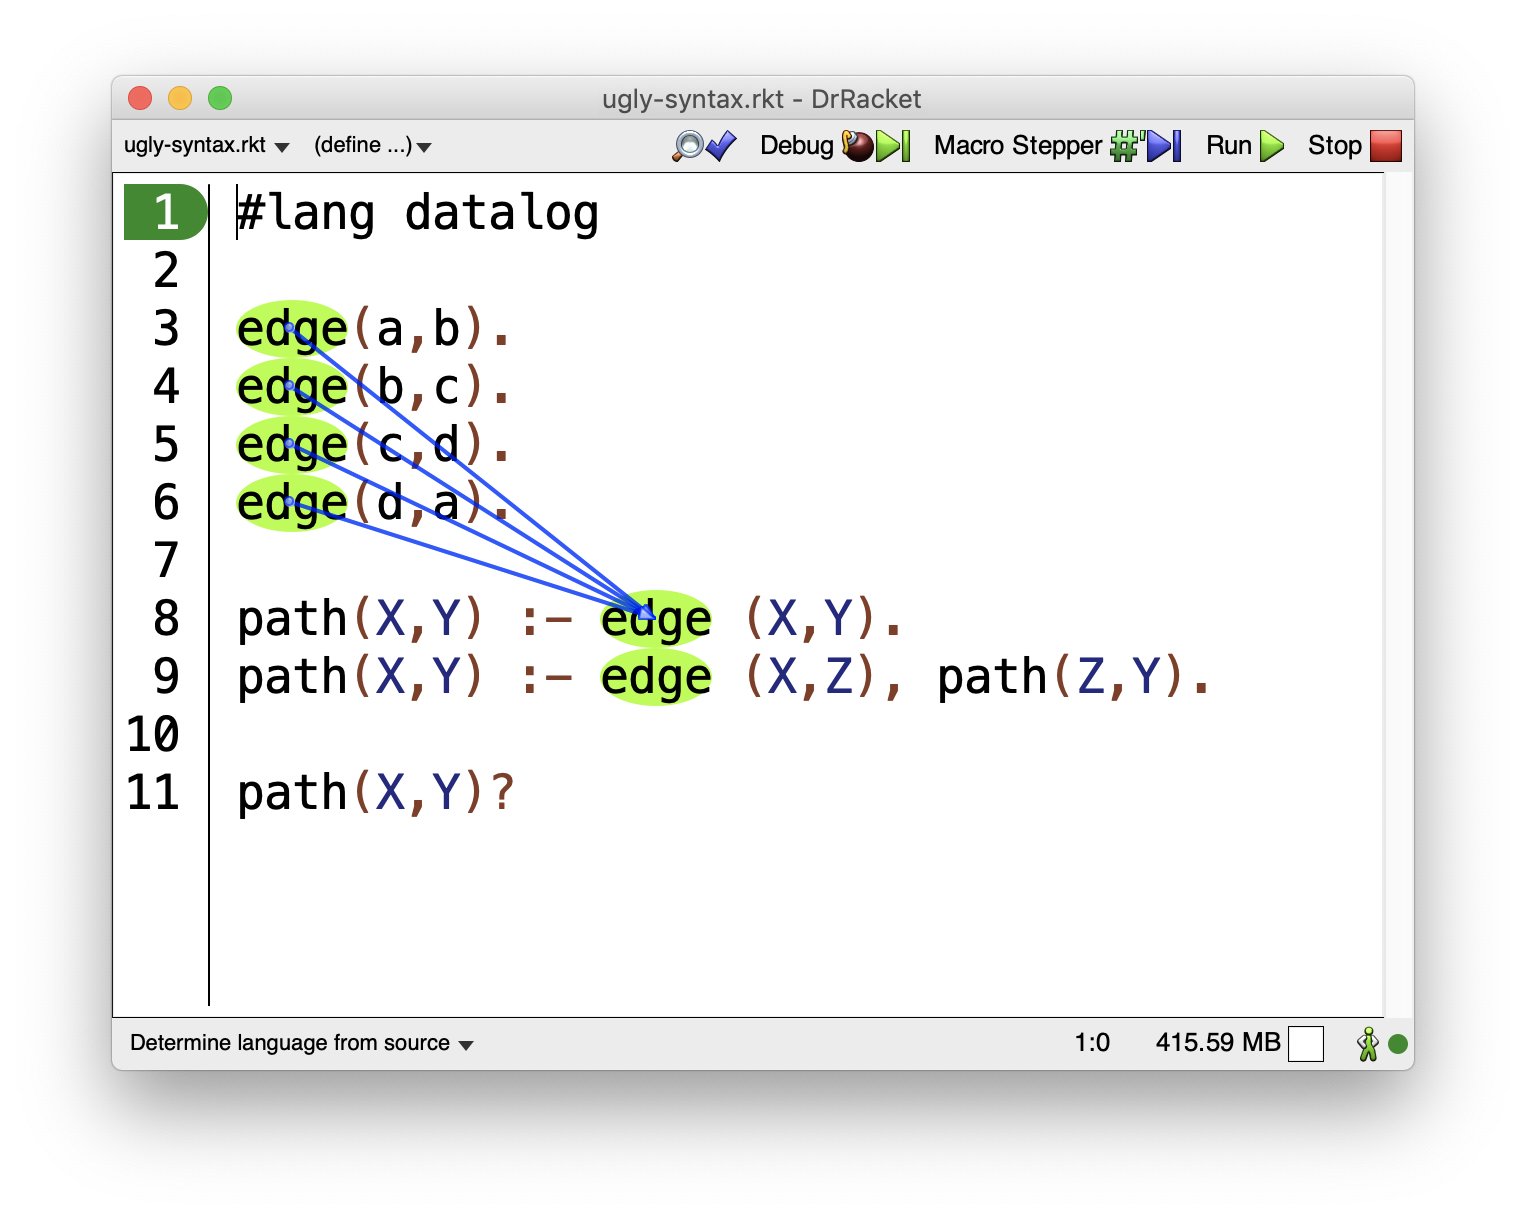
\includegraphics[]{images/racket-variable-arrow.png}
    \end{adjustbox}
    \caption{Результат интеграции языка datalog в IDE DrRacket.}\label{fig:racket-variable-arrow}
\end{figure}


\subsubsection{Структура программы}\label{sec:ch2/sec1/sub1/sub1}

Структура программы-описания аппаратного обеспечения имеет следующий вид, \cref{fig:device-program-structure}.

\begin{figure}[!htbp]
    \centering
    % !TEX encoding = UTF-8 Unicode
% Úτƒ-8 encoded
% http://www.linux.org.ru/forum/general/10357036
\tikzset{
    line/.style={draw, -latex'},
    every join/.style={line},
    u/.style={anchor=south},
    r/.style={anchor=west},
    fxd/.style={text width = 6em},
    it/.style={font={\small\itshape}},
    bf/.style={font={\small\bfseries}},
}
\tikzstyle{base_long} =
    [
        draw,
        on chain,
        on grid,
        align=center,
        minimum height=4ex,
        minimum width = 10ex,
        node distance = 6mm and 60mm,
        text badly centered,
    ]
\tikzstyle{base} =
    [
        draw,
        on chain,
        on grid,
        align=center,
        minimum height=4ex,
        minimum width = 10ex,
        node distance = 6mm and 60mm,
        text badly centered,
        text width=5cm
    ]
\tikzstyle{coord} =
    [
        coordinate,
        on chain,
        on grid
    ]
\tikzstyle{cloud} =
    [
        base,
        ellipse,
        node distance = 3cm,
        minimum height = 2em,
        text width=2cm
    ]
\tikzstyle{decision} =
    [
        base,
        diamond,
        aspect=2,
        node distance = 2cm,
        inner sep = 0pt
    ]
\tikzstyle{block} =
    [
        rectangle,
        base,
        rounded corners,
        minimum height = 2em
    ]
\tikzstyle{print_block} =
    [
        base,
        tape,
        tape bend top=none,
    ]
\tikzstyle{io} =
    [
        base,
        trapezium,
        trapezium left angle = 70,
        trapezium right angle = 110,
    ]
\tikzstyle{prompt} =
    [
        base,
        trapezium,
        trapezium left angle = 90,
        trapezium right angle = 80,
        shape border rotate = 90
    ]
\tikzstyle{disk file} =
    [
        base,
        cylinder,
        aspect=0.2,
    ]
\tikzstyle{process} =
    [
        rectangle,
        base,
    ]
\makeatletter
\pgfkeys{/pgf/.cd,
    subrtshape w/.initial=2mm,
    cycleshape w/.initial=2mm
}
\pgfdeclareshape{parallelshape}{
    \inheritsavedanchors[from=rectangle]
    \inheritanchorborder[from=rectangle]
    \inheritanchor[from=rectangle]{north}
    \inheritanchor[from=rectangle]{center}
    \inheritanchor[from=rectangle]{west}
    \inheritanchor[from=rectangle]{east}
    \inheritanchor[from=rectangle]{mid}
    \inheritanchor[from=rectangle]{base}
    \inheritanchor[from=rectangle]{south}
    \backgroundpath{
        \southwest \pgf@xa=\pgf@x \pgf@ya=\pgf@y
        \northeast \pgf@xb=\pgf@x \pgf@yb=\pgf@y
        \def\ppd@offset{\pgfpoint{\pgfutil@tempdima}{0ex}}
        \def\ppd@offsetm{\pgfpoint{-\pgfutil@tempdima}{0ex}}
        \pgfpathmoveto{\pgfqpoint{\pgf@xa}{\pgf@ya}}
            \pgfpathlineto{\pgfqpoint{\pgf@xb}{\pgf@ya}}
        \pgfpathclose
        \pgfpathmoveto{\pgfqpoint{\pgf@xb}{\pgf@yb}}
            \pgfpathlineto{\pgfqpoint{\pgf@xa}{\pgf@yb}}
        \pgfpathclose
    }
}
\pgfdeclareshape{subrtshape}{
    \inheritsavedanchors[from=rectangle]
    \inheritanchorborder[from=rectangle]
    \inheritanchor[from=rectangle]{north}
    \inheritanchor[from=rectangle]{center}
    \inheritanchor[from=rectangle]{west}
    \inheritanchor[from=rectangle]{east}
    \inheritanchor[from=rectangle]{mid}
    \inheritanchor[from=rectangle]{base}
    \inheritanchor[from=rectangle]{south}
    \backgroundpath{
        \southwest \pgf@xa=\pgf@x \pgf@ya=\pgf@y
        \northeast \pgf@xb=\pgf@x \pgf@yb=\pgf@y
        \pgfmathsetlength\pgfutil@tempdima{\pgfkeysvalueof{/pgf/subrtshape w}}
        \def\ppd@offset{\pgfpoint{\pgfutil@tempdima}{0ex}}
        \def\ppd@offsetm{\pgfpoint{-\pgfutil@tempdima}{0ex}}
        \pgfpathmoveto{\pgfqpoint{\pgf@xa}{\pgf@ya}}
        \pgfpathlineto{\pgfqpoint{\pgf@xb}{\pgf@ya}}
        \pgfpathlineto{\pgfqpoint{\pgf@xb}{\pgf@yb}}
        \pgfpathlineto{\pgfqpoint{\pgf@xa}{\pgf@yb}}
        \pgfpathclose
        \pgfpathmoveto{\pgfpointadd{\pgfpoint{\pgf@xa}{\pgf@yb}}{\ppd@offsetm}}
        \pgfpathlineto{\pgfpointadd{\pgfpoint{\pgf@xa}{\pgf@ya}}{\ppd@offsetm}}
        \pgfpathlineto{\pgfpointadd{\pgfpoint{\pgf@xb}{\pgf@ya}}{\ppd@offset}}
        \pgfpathlineto{\pgfpointadd{\pgfpoint{\pgf@xb}{\pgf@yb}}{\ppd@offset}}
        \pgfpathclose
    }
}
\pgfdeclareshape{cyclebegshape}{
    \inheritsavedanchors[from=rectangle]
    \inheritanchorborder[from=rectangle]
    \inheritanchor[from=rectangle]{north}
    \inheritanchor[from=rectangle]{center}
    \inheritanchor[from=rectangle]{west}
    \inheritanchor[from=rectangle]{east}
    \inheritanchor[from=rectangle]{mid}
    \inheritanchor[from=rectangle]{base}
    \inheritanchor[from=rectangle]{south}
    \backgroundpath{
        \southwest \pgf@xa=\pgf@x \pgf@ya=\pgf@y
        \northeast \pgf@xb=\pgf@x \pgf@yb=\pgf@y
        \pgfmathsetlength\pgfutil@tempdima{\pgfkeysvalueof{/pgf/cycleshape w}}
        \pgfpathmoveto{\pgfqpoint{\pgf@xa}{\pgf@ya}}
\pgfpathlineto{\pgfpointadd{\pgfpoint{\pgf@xa}{\pgf@yb}}{\pgfpoint{0ex}{-\pgfutil@tempdima}}}
\pgfpathlineto{\pgfpointadd{\pgfpoint{\pgf@xa}{\pgf@yb}}{\pgfpoint{\pgfutil@tempdima}{0ex}}}
\pgfpathlineto{\pgfpointadd{\pgfpoint{\pgf@xb}{\pgf@yb}}{\pgfpoint{-\pgfutil@tempdima}{0ex}}}
\pgfpathlineto{\pgfpointadd{\pgfpoint{\pgf@xb}{\pgf@yb}}{\pgfpoint{0ex}{-\pgfutil@tempdima}}}
\pgfpathlineto{\pgfqpoint{\pgf@xb}{\pgf@ya}}
        \pgfpathclose
    }
}
\pgfdeclareshape{cycleendshape}{
    \inheritsavedanchors[from=rectangle]
    \inheritanchorborder[from=rectangle]
    \inheritanchor[from=rectangle]{north}
    \inheritanchor[from=rectangle]{center}
    \inheritanchor[from=rectangle]{west}
    \inheritanchor[from=rectangle]{east}
    \inheritanchor[from=rectangle]{mid}
    \inheritanchor[from=rectangle]{base}
    \inheritanchor[from=rectangle]{south}
    \backgroundpath{
        \southwest \pgf@xa=\pgf@x \pgf@ya=\pgf@y
        \northeast \pgf@xb=\pgf@x \pgf@yb=\pgf@y
        \pgfmathsetlength\pgfutil@tempdima{\pgfkeysvalueof{/pgf/cycleshape w}}
        \pgfpathmoveto{\pgfqpoint{\pgf@xb}{\pgf@yb}}
\pgfpathlineto{\pgfpointadd{\pgfpoint{\pgf@xb}{\pgf@ya}}{\pgfpoint{0ex}{\pgfutil@tempdima}}}
\pgfpathlineto{\pgfpointadd{\pgfpoint{\pgf@xb}{\pgf@ya}}{\pgfpoint{-\pgfutil@tempdima}{0ex}}}
\pgfpathlineto{\pgfpointadd{\pgfpoint{\pgf@xa}{\pgf@ya}}{\pgfpoint{\pgfutil@tempdima}{0ex}}}
\pgfpathlineto{\pgfpointadd{\pgfpoint{\pgf@xa}{\pgf@ya}}{\pgfpoint{0ex}{\pgfutil@tempdima}}}
\pgfpathlineto{\pgfqpoint{\pgf@xa}{\pgf@yb}}
        \pgfpathclose
    }
}
\makeatother
\tikzstyle{subroutine} =
    [
        base,
        subrtshape,
    ]
\tikzstyle{cyclebegin} =
    [
        base,
        cyclebegshape,
    ]
\tikzstyle{cycleend} =
    [
        base,
        cycleendshape,
    ]
\tikzstyle{connector} =
    [
        base,
        circle,
    ]

\tikzstyle{parallel} =
    [
        base_long,
        parallelshape,
    ]
\begin{tikzpicture}[%
    start chain=going below,    % General flow is top-to-bottom
    node distance=6mm and 30mm, % Global setup of box spacing
    ]
        \node  [rectangle,
                base,
                minimum width=6cm] (device class)
                {Описание класса устройства};
        \node  [rectangle,
                base,
                minimum width=6cm] (c-python api)
                [below = 1.5cm of device class]
                {Связывание функций C-Python интерфейса};
        \node  [rectangle,
                base,
                minimum width=6cm] (py logic)
                [below = 1.85cm of c-python api]
                {Реализация логики работы устройства на Python};



\end{tikzpicture}

    \caption{Структура программы-описания аппаратного обеспечения.}\label{fig:device-program-structure}
\end{figure}

Несмотря на то, что компилятор язык программы-описания располагает
блоки кода в результирующем тексте модуле QEMU в соответствии
с правилами языка C и порядок объявления блоков в исходном файле ему не важен,
данная структура является наиболее понятной и органичной для стороннего разработчика.
Поэтому компилятор принуждает программиста придерживаться её, подобно тому, как
язык Python обязывает использовать отступы для создания блоков кода.

\section{Формализация задачи}\label{sec:ch2/sec2/sub1}

\subsection{Граммматика языка}\label{sec:ch2/sec2/sub2}
Разрабатываемый язык является языком с контекстно-свободной грамматикой.
Далее он будет именоваться как {\mylanguage} (произносится \mylanguageprononciation)

Грамматика {\mylanguage} ограничена до описания зависимостей устройства и QEMU,
связывания функций C и Python, встраивания Python-кода с логикой работы устройства
в файл.


% TODO: Учтено ли, что пользователь захочет кастомизировать функции инициализации класса и инстанса?
% TODO: MemoryRegionOps?
\setlength{\grammarparsep}{0.1cm}
\setlength{\grammarindent}{13em}
\begin{figure}[!htbp]
    \begin{grammar}
        <letter> ::= `a' ... `z' | `A' ... `Z';

        <digit> ::= `0' ... `9' ;

        <symbol> ::= \symbol{92}x20 ... \symbol{92}x7E ; (* любой печатный символ, согласно кодам ASCII *)

        <const value> ::= <digit> | `"' \{ <symbol> \} `"';

        <identifier> ::= <letter> [\{ <letter> | <digit> | `\_' \}] ;

        <block start> ::= `{';

        <block end> ::= `}';

        <field> ::= <identifier> `=' <identifier> | <block> ;

        <block> ::= <block start> <field> [\{ `,' <field> \}] <block end>;

        <device definition> ::= '\#' <identifier>;

        <device class inheritance> ::= `(' <identifier> `:' <identifier> [\{ `,' <identifier> \}] `)';

        <device class block> ::= <device class inheritance> <block>;

        <bind block> ::= `@bind' <block>;

        <python block> ::= `@py' <block>;

        <program> ::= <device definition> <device class block> <bind block> <python block>;
    \end{grammar}
    \caption{Расширенная форма Бэкуса-Наура \mylanguage}\label{fig:qpydev-grammar}
\end{figure}


\subsection{Семантика языка}\label{sec:ch2/sec2/sub3}

Для описания семантики языка {\mylanguage} была выбрана денотационная семантика, \cref{table:denotational-semantics}.
Краеугольным камнем денотационной семантики является определение для каждой сущности
языка некоего математического объекта и некоей функции, называемой интерпретатором,
которая отображает экземпляры этой сущности в экземпляры этого математического объекта -- элемент множества денотаций.
Поскольку математические объекты строго определены, то они представляют собой точный
смысл соответствующих сущностей.

Функции обозначают посредством двойных квадратных скобок $[[$ $]]$,
а элемент алгебры или операция алгебры, сопоставленные функцией $[[$ $]]$
правильному выражению или конструктору выражений, называют денотантом этого выражения или,
соответственно, денотацией конструкции. \cite{denotational-semantics}

Для языка {\mylanguage} значимыми множествами семантических объектов
являются только множества $Q$ -- объектов QEMU (переменные, функции, структуры) и
$C$ -- множество константных выражений.


\renewcommand*{\arraystretch}{1.5}
\begin{longtable}{| c | p{6cm} |}
    \caption{Денотационная семантика {\mylanguage}}\label{table:denotational-semantics} \\
    \hline
    \text{Математическое описание} & \multicolumn{1}{|c|}{Значение} \\
    \hline
    $[[assignment]](x,y) = \lambda x.y$
    & Операция присваивания значения $y$ переменной $x$ \\
    \hline
    \makecell{$[[terminate]](m) =$\\ \text{Завершение работы компилятора}}
    & Терминирование компилятора \\
    \hline
    $[[if]](c,e_1,e_2) =
    \begin{cases}
        e_1, & \text{Если } c = true \\
        e_2, & \text{Если } c \not= true
    \end{cases}$
    & Условное исполнение. Если условие $c$ истинно, то
    выполняется $e_1$, иначе $e_2$ \\
    \hline
    $[[throw\ error]](c, e) = if(c, e_g, terminate)$
    & Создание и бросание исключения при ложном условии $c$ \\
    \hline
    $[[lookup]](o) = [[throw\ error]](o \in Q, o)$
    & Поиск объекта $o$ в множестве объектов QEMU $Q$.
    В случае, если объект не найден генерируется исключение \\
    \hline
    $[[<device\ definition>]](i) = lookup(i)$
    & Поиск указнного класса устройства в объектах QEMU \\
    \hline
    \makecell{$[[<device\ class\ inheritance>]](i_1,...,i_n) = $\\
              $lookup(i_1) \land ... \land lookup(i_n)$}
    & Поск указанного класса для наследования и интерфейсов
    в объектах QEMU. Для успешного завершения должны быть
    найдены все объекты \\
    \hline
    \makecell{$[[<field>]](v_1, v_2) = $\\
              $[[throw\ error]](v_1 \in Q \land v_2 \in C \cup Q,$\\
              $assignment(v_1, v_2))$}
    & Присваивание полям значений при условии, что $v_1$
    принадлежит множеству объектов QEMU, а $v_2$ множеству
    констант или множеству объектов QEMU \\
    \hline
    $[[<block>]](f_1,...,f_n) = field(f_1) \land ... \land field(f_n)$
    & Присваивание связанных с одной сущностью полей \\
    \hline
    $[[<python block>]](b) = assignment(B,B)$ & \\
    \hline
\end{longtable}


\section{Поиск используемых сущностей QEMU}\label{sec:ch2/sec2}

Пробрасывание -- процесс преобразовывания и передачи данных между двумя интерфейсами.

Поиск используемых сущностей состоит в установлении типов QEMU для последующего
корректного пробрасывания их в логику устройства.
Также это необходимо для проверки корректности наследования и встраивания устройства.
Необходимыми для пробрасывания типами являются структуры и функции, оперирующие ими.

Рекурсивное преобразование структур QEMU в типы python важно для удобного и читаемого
использования C-объектов внутри python-логики.
Пробрасывание в python функций QEMU необходимо для использования уже имеющегося API эмулятора.
% TODO: может удалить, если это сложно
Потенциально, может быть удобным использование макросов препроцессора C внутри
логики Python.

\subsection{Механизм нахождения информации о типах устройств}\label{sec:ch2/sec2/sub2/sub1}

Все устройства QEMU:
\begin{enumerate}[label={\arabic*)}]
    \item имеют родителя и распределены по подпапкам папки \texttt{hw};
    \item объявляют структуру \texttt{TypeInfo}, в которой указывается родитель устройства
          и размер создаваемого объекта -- поле \texttt{.instance\_size}
          (используется для создания объектов устройств на системной шине);
    \item используют оператор \texttt{sizeof},
          передавая ему имя структуры устройства, которое будет исполняться в QEMU.
\end{enumerate}

Данная информация позволяет найти используемые сущности QEMU следующим образом:
\begin{enumerate}[label={\arabic*)}]
    \item пройтись по всем файлам, находящимся в папке \texttt{hw};
    \begin{enumerate}[label={\arabic*)}]
        \item найти структуру \texttt{TypeInfo};
        \item проанализировать поле \texttt{.instance\_size} и сохранить
              используемую структуру как возможную для наследования;
        \item сохранить поле \texttt{.name} в качестве имени структуры для наследования;
    \end{enumerate}
\end{enumerate}

Помимо явного описания структуры \texttt{TypeInfo} некоторые устройства, написанные
в современном стиле, используют макросы:
\begin{enumerate}[label={\arabic*)}]
    \item \label{main-def-macro} \texttt{OBJECT\_DEFINE\_TYPE\_EXTENDED};
    \item \texttt{OBJECT\_DEFINE\_TYPE};
    \item \texttt{OBJECT\_DEFINE\_TYPE\_WITH\_INTERFACES};
    \item \texttt{OBJECT\_DEFINE\_ABSTRACT\_TYPE}.
\end{enumerate}

Все перечисленные макросы создают структуру \texttt{TypeInfo} и все, кроме\cref{main-def-macro},
вызывают внутри себя макрос\cref{main-def-macro}, специализируя определенные поля структуры \texttt{TypeInfo}.
Например \texttt{OBJECT\_DEFINE\_ABSTRACT\_TYPE} создает абстрактный тип, передавая внутри себя
значение \texttt{true} макросу \texttt{OBJECT\_DEFINE\_TYPE\_EXTENDED}, чем облегчает собственный интерфейс
и делает свое использование более выразительным.

Список аргументов макросов объявления типов также требуется разбирать, чтобы получить из аргументов информацию
о структуре \texttt{TypeInfo}.

Механизм получения информации о функциях намного проще: в языке C функции могут инкапсулироваться
только на уровне одного модуля трансляции -- C-файла, прошедшего этап препроцессирования.
Инкапсулированные функции помечаются ключевым словом \texttt{static}, что делает их
<<невидимыми>> в других модулях трансляции.
Все функции, не помеченные ключевым словом \texttt{static} будем считать интерфейсными.

Данная информация будет использована впоследствии для корректной кодогенерации устройства
и преобразования C-структур и C-функций в читаемый вид для python-интерфейса.

\subsection{Механизм использования информации о типах устройств}\label{sec:ch2/sec2/sub2/sub2}

Так как код QEMU насыщен использованием макросов, потребуется инструмент для их разворачивания -- препроцессор.
Чтобы не создавать собственную имплементацию препроцессора, этим будет заниматься препоцессор системного компилятора.

Практически во всех системах сборки программ в POSIX окружении используется компилятор gcc или clang.
Оба компилятора являются совместимыми между собой. Для задействования препроцессора компилятора используется
опция \texttt{-E}. Так как препроцессор C, помимо раскрытия макросв занимается еще нахождением и подстановкой
заголовочных файлов, то потребуется указать папки с их местонахождением.
QEMU полагается на:
\begin{enumerate}[label={\arabic*)}]
    \item \label{build-header} заголовочные файлы, создаваемые в процессе сборки эмулятора;
    \item библиотеку GLib;
    \item заголовочные файлы, находящиеся в папке \texttt{include}.
\end{enumerate}

Так как файлы в пункте\cref{build-header} появляются в процессе сборки, то конкретную версию QEMU нужно будет собрать.
Сборка также полезна, так как в процессе конфигурации эмулятора выставляются определенные переменные
препроцессора (дефайны -- от директивы \texttt{\#define}), которые влияют на условные выражения
препроцессора, а те, в свою очередь, на генерацию исходного кода.
Использование в данном случае статического анализатора кода было бы затруднительным, так как
информация о конкретной конфигурации не может быть получена без непосредственной сборки.

Укзание папки для препроцессора производится с помощью опции \texttt{-I}.
\begin{lstlisting}[caption={Пример строки запуска препроцессора для определенного файла устройства},
                   captionpos=b]
gcc -E hw/misc/edu.c
    -I ./include/
    -I ./build/
    -I/usr/include/glib-2.0
    -I/usr/lib64/glib-2.0/include
\end{lstlisting}


\section{Генерация python-интерфейса для логики устройства}\label{sec:ch2/sec2/sub3}

% TODO: как это вяжется со SWIG'ом?
Определение интерфейса используемых сущностей QEMU происходит в уже препроцессированном коде\cref{sec:ch2/sec2/sub2/sub2}.
Python, в эталонной реализации, является интерпретируемым языком программирования со сборщиком мусора.
Python спользует для сбора мусора подсчет ссылок и поколенческий сборщик мусора, чей API описан в модуле \texttt{gc}.
Уничтожение объектов, основанное на подсчете ссылок использует простое правило: если на объект больше
никто не ссылается, то память, занимаемая объектом, высвобождается.
Классическим недостатком данного подхода являются циклические ссылки: если объект \textit{A} ссылается
на объект \textit{B} (или же сам на себя), а тот, в свою очередь ссылается на объект \textit{A}, то система, основанная
только на подсчете ссылок, не может определить, реально ли используются оба этих объекта или нет.
В зависимости от языка, принимаются различные меры противодействия данной ситуации
(например Perl 5 никак не детектирует циклические ссылки между объектами,
из-за чего занимаемая ими память возвращается операционной системе только в момент завершения
работы интерпретатора).
В Python для решения данной проблемы используется поколенческий сборщик мусора (generational garbage collector),
который переодически запускается. Сборщик мусора выделяет три поколения объектов,
различающихся интервалами сканирования на предмет <<мусора>>:
\begin{itemize}
    \item первое поколение -- в него попадают все новые объекты;
    \item второе поколение -- если объект выжил после сборки мусора
        в первом поколении, то он перемещается во второе;
    \item третье поколение проверяется на наличие мусора только когда
        соотношение $\frac{\text{объекты, перемещаемые в верхнее поколение}}{\text{количество объектов второго и третьего поколения}} > 25\%$;
\end{itemize}

Тогда как поколенческий сборщик мусора можно отключить, подсчет ссылок нельзя, он ведется автоматически
для Python-кода и вручную C-кода с помощью макросов \texttt{Py\_INCREF} и \texttt{Py\_XINCREF}
увеличивают счетчик ссылок на объект, \texttt{Py\_DECREF} и \texttt{Py\_XDECREF}.
Разница между \texttt{X}-макросами и обычными состоит в том, что \texttt{X}-макросы
проверяют равенство передаваемого указателя \texttt{NULL}, из-за чего исполняются дольше.
Если указатель нулевой, то макрос ничего не делает.
Использование \texttt{Py\_DECREF} или \texttt{Py\_INCREF} на \texttt{NULL} приведет к ошибке во время исполнения.
Помимо этого нужно иметь в виду, что \texttt{Py\_DECREF} (и \texttt{Py\_XDECREF}) могут потенциально
привести к исполнению произвольного кода на Python, так как, в случае обнуления счетчика
ссылок у объектов, для которых определен деструктор (например освобождающий подключение к базе данных),
перед удалением объекта он будет вызван.


\subsection{Генерация Python-интерфейса для C-кода}\label{sec:ch2/sec2/sub3/sub1}

Язык Python является скорее интерфейсом, чем языком программирования:
документация описывает то, какие функции и конструкции должен предоставлять язык, чтобы являться Python'ом.
Подтверждением этому служит большое количество различных реализаций языка, например:
\begin{itemize}
    \item IronPython/Jython -- интерпретатор, работающий в CLR и JVM соответственно;
    \item PyPy -- JIT-интерпретатор, изначально написанный на самом Python;
    \item CPython -- эталонный интерпретатор Python, написанный на языке C;
\end{itemize}

Под языком Python практически всегда понимается интерпретатор CPython, как раз его
API для создания связки между кодом на C и Python и будет использоваться.

Для создания бесшовной интеграции, требуется:
\begin{itemize}
    \item преобразовывать C-структуры и C-функции в Python-объекты;
    \item оборачивать C-функции для конвертации Python-аргументов в C-типы;
    \item транслировать изменения связанных объектов внутри Python-кода.
\end{itemize}

\paragraph{SWIG} --  Simplified Wrapper and Interface Generator.
Данное ПО позволяет автоматически генерировать обертки над C/C++ библиотеками для
большого спектра высокоуровневых языков программирования (\cref{fig:swig}).
Для этого требуется написать интерфейсный файл, в котором будут описаны шаблоны
функций и структур, для которых требуется сгенерировать интерфейс.
SWIG принимает на вход файл с описанием шаблонов для нахождения структур и
функций, которые будут экспортированы в межъязыковой интерфейс.
Несмотря на удобство, SWIG не обладает возможностями препроцессора и понимает
только ограниченное количество его директив, причем \texttt{define}'ы воспринимает
только если они объявляют константы.

\begin{figure}[!htbp]
    \centering
    \begin{adjustbox}{max totalsize={0.8\textwidth}{\textheight}}
        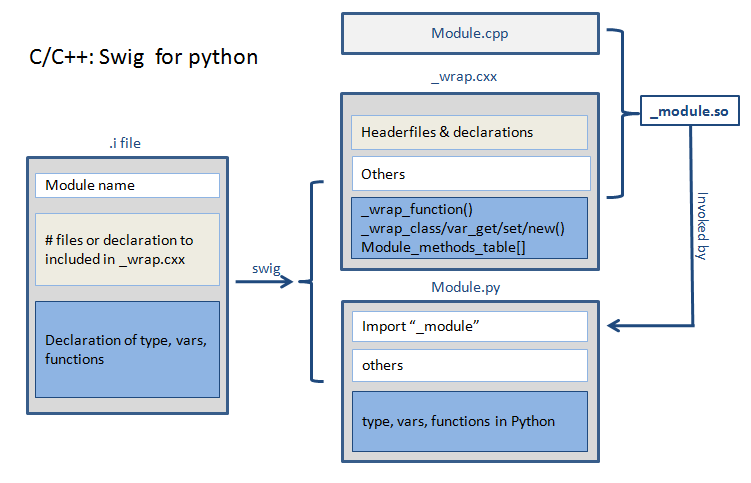
\includegraphics[]{images/swig.png}
    \end{adjustbox}
    \caption{Схема работы SWIG.}\label{fig:swig}
\end{figure}

Исходя из этого и того, что SWIG генерирует очень большое количество кода,
который все равно придется дополнять обращениями к C-API Python то логичнее
реализовать свое нахождение и преобразование C-сущностей.

Для этого используется пакет c-utils \cite{c-utils} для языка Racket.
В нем реализован разбор грамматики, с учетом всех особенностей
языка: в C имеется два лексических класса, которые считаются
отличными в грамматике, но их использование идентично.
Это типы и их псевдонимы, задаваемые ключевым словом \texttt{typedef}.
Язык различает два этих класса по их связке с типом, поэтому
парсерам приходится поддерживать внутреннее окружение и предоставлять
его лексеру \cite{c-utils-internals}.

В Python существует несколько способов импорта C-сущностей:

\begin{enumerate}[label={\arabic*)}]
    \item \texttt{PyCapsule} -- позволяет инкапсулировать и передавать данные, находящиеся по некому указателю
          сквозь Python-код обратно в C. Сам Python не имеет доступа к инкапсулированному объекту
          так как не сохраняет никакой информации о типе. Ограничением в использовании \texttt{PyCapsule}
          является невозможность работы с данным объектом из многопоточного кода, так как
          Python не может его сериализовать;
    \item \texttt{memoryview} -- созданные объекты являются <<отображениями>> памяти, дают доступ
          к некоторому C-буферу, обозначенному при создании объекта. Можно использовать для
          экспорта сущностей, но с перекладыванием ответственности на интерпретацию байтов буфера
          на Python-код;
    \item Создание Python-объекта, отражающего C-сущность. Можно выполнить отдельным классом или
          же словарем.
\end{enumerate}

В {\mylanguage} для C-сущностей генерируются классы (\cref{fig:py-api-compilation}), отражающие их внутреннее устройство.
Объекты классов не имеют полей, и могут быть использованы только через оператор \texttt{[]}.
В пардигме Python, данный оператор является <<синтаксическим сахаром>> для вызова <<магических>>
функций \texttt{\_\_setitem\_\_} для выставления поля и \texttt{\_\_getitem\_\_} для получения значения.
В данном случае для \texttt{\_\_setitem\_\_} и \texttt{\_\_getitem\_\_} согласно C-API \cite{python-c-type-objects}
генерируются функции, которые первым делом производят конвертацию Python-типов в C-типы,
после чего уже возвращают или выставляют сконвертированные значения в структуры (листинг\cref{lst:python-c-type-objects}).

\begin{lstlisting}[caption={Пример доступа к элементу структуры из Python.},
                   captionpos=b,
                   language=python]
# вызывается функция __getitem__, которая по возможности
# конвертирует C-тип в Python-тип и возвращает Python-сущность,
# присваивая её переменной source.
source = EduState["dma_state"]["src"]

# вызывается функция __setitem__, которая по возможности
# конвертирует Python-тип в C-тип, после чего
# полю EduState.dma_state.dst присваивается значение.
EduState["dma_state"]["dst"] = source + 0x1234
\end{lstlisting}\label{lst:python-c-type-objects}

\begin{figure}[!htbp]
    \centering
    \hspace*{-11cm}
    \scalebox{0.8}{
        \begin{minipage}{10cm}
            % !TEX encoding = UTF-8 Unicode
% Úτƒ-8 encoded
% http://www.linux.org.ru/forum/general/10357036
\tikzset{
    line/.style={draw, -latex'},
    every join/.style={line},
    u/.style={anchor=south},
    r/.style={anchor=west},
    fxd/.style={text width = 6em},
    it/.style={font={\small\itshape}},
    bf/.style={font={\small\bfseries}},
}
\tikzstyle{base_long} =
    [
        draw,
        on chain,
        on grid,
        align=center,
        minimum height=4ex,
        minimum width = 10ex,
        node distance = 6mm and 60mm,
        text badly centered,
    ]
\tikzstyle{base} =
    [
        draw,
        on chain,
        on grid,
        align=center,
        minimum height=4ex,
        minimum width = 10ex,
        node distance = 6mm and 60mm,
        text badly centered,
        text width=5cm
    ]
\tikzstyle{coord} =
    [
        coordinate,
        on chain,
        on grid
    ]
\tikzstyle{cloud} =
    [
        base,
        ellipse,
        node distance = 3cm,
        minimum height = 2em,
        text width=2cm
    ]
\tikzstyle{decision} =
    [
        base,
        diamond,
        aspect=2,
        node distance = 2cm,
        inner sep = 0pt
    ]
\tikzstyle{block} =
    [
        rectangle,
        base,
        rounded corners,
        minimum height = 2em
    ]
\tikzstyle{print_block} =
    [
        base,
        tape,
        tape bend top=none,
    ]
\tikzstyle{io} =
    [
        base,
        trapezium,
        trapezium left angle = 70,
        trapezium right angle = 110,
    ]
\tikzstyle{prompt} =
    [
        base,
        trapezium,
        trapezium left angle = 90,
        trapezium right angle = 80,
        shape border rotate = 90
    ]
\tikzstyle{disk file} =
    [
        base,
        cylinder,
        aspect=0.2,
    ]
\tikzstyle{process} =
    [
        rectangle,
        base,
    ]
\makeatletter
\pgfkeys{/pgf/.cd,
    subrtshape w/.initial=2mm,
    cycleshape w/.initial=2mm
}
\pgfdeclareshape{parallelshape}{
    \inheritsavedanchors[from=rectangle]
    \inheritanchorborder[from=rectangle]
    \inheritanchor[from=rectangle]{north}
    \inheritanchor[from=rectangle]{center}
    \inheritanchor[from=rectangle]{west}
    \inheritanchor[from=rectangle]{east}
    \inheritanchor[from=rectangle]{mid}
    \inheritanchor[from=rectangle]{base}
    \inheritanchor[from=rectangle]{south}
    \backgroundpath{
        \southwest \pgf@xa=\pgf@x \pgf@ya=\pgf@y
        \northeast \pgf@xb=\pgf@x \pgf@yb=\pgf@y
        \def\ppd@offset{\pgfpoint{\pgfutil@tempdima}{0ex}}
        \def\ppd@offsetm{\pgfpoint{-\pgfutil@tempdima}{0ex}}
        \pgfpathmoveto{\pgfqpoint{\pgf@xa}{\pgf@ya}}
            \pgfpathlineto{\pgfqpoint{\pgf@xb}{\pgf@ya}}
        \pgfpathclose
        \pgfpathmoveto{\pgfqpoint{\pgf@xb}{\pgf@yb}}
            \pgfpathlineto{\pgfqpoint{\pgf@xa}{\pgf@yb}}
        \pgfpathclose
    }
}
\pgfdeclareshape{subrtshape}{
    \inheritsavedanchors[from=rectangle]
    \inheritanchorborder[from=rectangle]
    \inheritanchor[from=rectangle]{north}
    \inheritanchor[from=rectangle]{center}
    \inheritanchor[from=rectangle]{west}
    \inheritanchor[from=rectangle]{east}
    \inheritanchor[from=rectangle]{mid}
    \inheritanchor[from=rectangle]{base}
    \inheritanchor[from=rectangle]{south}
    \backgroundpath{
        \southwest \pgf@xa=\pgf@x \pgf@ya=\pgf@y
        \northeast \pgf@xb=\pgf@x \pgf@yb=\pgf@y
        \pgfmathsetlength\pgfutil@tempdima{\pgfkeysvalueof{/pgf/subrtshape w}}
        \def\ppd@offset{\pgfpoint{\pgfutil@tempdima}{0ex}}
        \def\ppd@offsetm{\pgfpoint{-\pgfutil@tempdima}{0ex}}
        \pgfpathmoveto{\pgfqpoint{\pgf@xa}{\pgf@ya}}
        \pgfpathlineto{\pgfqpoint{\pgf@xb}{\pgf@ya}}
        \pgfpathlineto{\pgfqpoint{\pgf@xb}{\pgf@yb}}
        \pgfpathlineto{\pgfqpoint{\pgf@xa}{\pgf@yb}}
        \pgfpathclose
        \pgfpathmoveto{\pgfpointadd{\pgfpoint{\pgf@xa}{\pgf@yb}}{\ppd@offsetm}}
        \pgfpathlineto{\pgfpointadd{\pgfpoint{\pgf@xa}{\pgf@ya}}{\ppd@offsetm}}
        \pgfpathlineto{\pgfpointadd{\pgfpoint{\pgf@xb}{\pgf@ya}}{\ppd@offset}}
        \pgfpathlineto{\pgfpointadd{\pgfpoint{\pgf@xb}{\pgf@yb}}{\ppd@offset}}
        \pgfpathclose
    }
}
\pgfdeclareshape{cyclebegshape}{
    \inheritsavedanchors[from=rectangle]
    \inheritanchorborder[from=rectangle]
    \inheritanchor[from=rectangle]{north}
    \inheritanchor[from=rectangle]{center}
    \inheritanchor[from=rectangle]{west}
    \inheritanchor[from=rectangle]{east}
    \inheritanchor[from=rectangle]{mid}
    \inheritanchor[from=rectangle]{base}
    \inheritanchor[from=rectangle]{south}
    \backgroundpath{
        \southwest \pgf@xa=\pgf@x \pgf@ya=\pgf@y
        \northeast \pgf@xb=\pgf@x \pgf@yb=\pgf@y
        \pgfmathsetlength\pgfutil@tempdima{\pgfkeysvalueof{/pgf/cycleshape w}}
        \pgfpathmoveto{\pgfqpoint{\pgf@xa}{\pgf@ya}}
\pgfpathlineto{\pgfpointadd{\pgfpoint{\pgf@xa}{\pgf@yb}}{\pgfpoint{0ex}{-\pgfutil@tempdima}}}
\pgfpathlineto{\pgfpointadd{\pgfpoint{\pgf@xa}{\pgf@yb}}{\pgfpoint{\pgfutil@tempdima}{0ex}}}
\pgfpathlineto{\pgfpointadd{\pgfpoint{\pgf@xb}{\pgf@yb}}{\pgfpoint{-\pgfutil@tempdima}{0ex}}}
\pgfpathlineto{\pgfpointadd{\pgfpoint{\pgf@xb}{\pgf@yb}}{\pgfpoint{0ex}{-\pgfutil@tempdima}}}
\pgfpathlineto{\pgfqpoint{\pgf@xb}{\pgf@ya}}
        \pgfpathclose
    }
}
\pgfdeclareshape{cycleendshape}{
    \inheritsavedanchors[from=rectangle]
    \inheritanchorborder[from=rectangle]
    \inheritanchor[from=rectangle]{north}
    \inheritanchor[from=rectangle]{center}
    \inheritanchor[from=rectangle]{west}
    \inheritanchor[from=rectangle]{east}
    \inheritanchor[from=rectangle]{mid}
    \inheritanchor[from=rectangle]{base}
    \inheritanchor[from=rectangle]{south}
    \backgroundpath{
        \southwest \pgf@xa=\pgf@x \pgf@ya=\pgf@y
        \northeast \pgf@xb=\pgf@x \pgf@yb=\pgf@y
        \pgfmathsetlength\pgfutil@tempdima{\pgfkeysvalueof{/pgf/cycleshape w}}
        \pgfpathmoveto{\pgfqpoint{\pgf@xb}{\pgf@yb}}
\pgfpathlineto{\pgfpointadd{\pgfpoint{\pgf@xb}{\pgf@ya}}{\pgfpoint{0ex}{\pgfutil@tempdima}}}
\pgfpathlineto{\pgfpointadd{\pgfpoint{\pgf@xb}{\pgf@ya}}{\pgfpoint{-\pgfutil@tempdima}{0ex}}}
\pgfpathlineto{\pgfpointadd{\pgfpoint{\pgf@xa}{\pgf@ya}}{\pgfpoint{\pgfutil@tempdima}{0ex}}}
\pgfpathlineto{\pgfpointadd{\pgfpoint{\pgf@xa}{\pgf@ya}}{\pgfpoint{0ex}{\pgfutil@tempdima}}}
\pgfpathlineto{\pgfqpoint{\pgf@xa}{\pgf@yb}}
        \pgfpathclose
    }
}
\makeatother
\tikzstyle{subroutine} =
    [
        base,
        subrtshape,
    ]
\tikzstyle{cyclebegin} =
    [
        base,
        cyclebegshape,
    ]
\tikzstyle{cycleend} =
    [
        base,
        cycleendshape,
    ]
\tikzstyle{connector} =
    [
        base,
        circle,
    ]

\tikzstyle{parallel} =
    [
        base_long,
        parallelshape,
    ]
\begin{tikzpicture}[%
    start chain=going below,    % General flow is top-to-bottom
    node distance=6mm and 30mm, % Global setup of box spacing
    ]
        \node [disk file] (qemu parent source) at (0,0) {\small Исходный код родительского устройства};
        \node [process]   (preprocessor) [right = 8cm of qemu parent source] {\small Препроцессор языка C};
        \node [subroutine] (c-utils) [below = 2cm of preprocessor] {\small Парсер языка C};
        \node [cyclebegin] (struct analysis) [below = 2cm of c-utils] {\small Пока есть поля в структуре};

        \node [decision] (is field another struct) [below = 4cm of struct analysis]
                         {\small Поле является \\ структурой \\или указателем \\ на структуру?};

        \node [block] (create python type) [below = 4cm of is field another struct] {\small Создание python-типа};

        \node [cycleend] (struct analysis end) [below = 2cm of create python type] {\small Пока есть поля в структуре};
        \node [disk file] (result) [below = 3cm of struct analysis end] {\small Результирующий файл интерфейса};


        \node [block] (python type C-API) [below left = 13cm of is field another struct,
                                           minimum width = 8cm,
                                           align = left,
                                           text width=10cm]
            {
            \begin{lstlisting}[language=c,
                                basicstyle=\tiny,
                                breakatwhitespace=true,
                                numbers=none,
                                keywordstyle=\color{blue},
                                otherkeywords = {uint32_t, bool, PyObject}]

PyObject* CustomDevice_get_item(PyObject *o, PyObject *key){
    char *field = NULL;
    PyArg_ParseTuple(key, "s", field);
    if(!strcmp(field, "...")){
    ...
    }
    elif (!strcmp(field, "...")){
    ...
    }
}
typedef struct {
    PyObject_HEAD
    uint32_t addr;
    bool busy;
    ...
} CustomDevice;
             \end{lstlisting}
            };

        \draw [->] (qemu parent source) -- (preprocessor);
        \draw [->] (preprocessor) -- (c-utils);
        \draw [->] (c-utils) -- (struct analysis);
        \draw [->] (struct analysis) -- (is field another struct);
        \draw [->] (is field another struct.east) -- (12.8, -2) -- (10.88, -2) node [midway, above, sloped] (yes) {Да};
        \draw [->] (is field another struct) -- (create python type) node [midway, above, sloped] (no) {Нет};
        \draw [->] (create python type) -- (struct analysis end);
        \draw [->] (struct analysis end) -- (result);

        \draw [dotted] (create python type.south west) -- (python type C-API.south east);
        \draw [dotted] (create python type.north west) -- (python type C-API.north west);


\end{tikzpicture}

        \end{minipage}
    }
    \caption{Схема создания Python-сущностей для структур QEMU.}\label{fig:py-api-compilation}
\end{figure}

Создание функций, обращающихся к Python-логике тривиальнее, так как их создание следует
линейному алгоритму (\cref{fig:py-api-func-gen-algo-compilation}).

\begin{figure}[!htbp]
    \centering
    % !TEX encoding = UTF-8 Unicode
% Úτƒ-8 encoded
% http://www.linux.org.ru/forum/general/10357036
\tikzset{
    line/.style={draw, -latex'},
    every join/.style={line},
    u/.style={anchor=south},
    r/.style={anchor=west},
    fxd/.style={text width = 6em},
    it/.style={font={\small\itshape}},
    bf/.style={font={\small\bfseries}},
}
\tikzstyle{base_long} =
    [
        draw,
        on chain,
        on grid,
        align=center,
        minimum height=4ex,
        minimum width = 10ex,
        node distance = 6mm and 60mm,
        text badly centered,
    ]
\tikzstyle{base} =
    [
        draw,
        on chain,
        on grid,
        align=center,
        minimum height=4ex,
        minimum width = 10ex,
        node distance = 6mm and 60mm,
        text badly centered,
        text width=5cm
    ]
\tikzstyle{coord} =
    [
        coordinate,
        on chain,
        on grid
    ]
\tikzstyle{cloud} =
    [
        base,
        ellipse,
        node distance = 3cm,
        minimum height = 2em,
        text width=2cm
    ]
\tikzstyle{decision} =
    [
        base,
        diamond,
        aspect=2,
        node distance = 2cm,
        inner sep = 0pt
    ]
\tikzstyle{block} =
    [
        rectangle,
        base,
        rounded corners,
        minimum height = 2em
    ]
\tikzstyle{print_block} =
    [
        base,
        tape,
        tape bend top=none,
    ]
\tikzstyle{io} =
    [
        base,
        trapezium,
        trapezium left angle = 70,
        trapezium right angle = 110,
    ]
\tikzstyle{prompt} =
    [
        base,
        trapezium,
        trapezium left angle = 90,
        trapezium right angle = 80,
        shape border rotate = 90
    ]
\tikzstyle{disk file} =
    [
        base,
        cylinder,
        aspect=0.2,
    ]
\tikzstyle{process} =
    [
        rectangle,
        base,
    ]
\makeatletter
\pgfkeys{/pgf/.cd,
    subrtshape w/.initial=2mm,
    cycleshape w/.initial=2mm
}
\pgfdeclareshape{parallelshape}{
    \inheritsavedanchors[from=rectangle]
    \inheritanchorborder[from=rectangle]
    \inheritanchor[from=rectangle]{north}
    \inheritanchor[from=rectangle]{center}
    \inheritanchor[from=rectangle]{west}
    \inheritanchor[from=rectangle]{east}
    \inheritanchor[from=rectangle]{mid}
    \inheritanchor[from=rectangle]{base}
    \inheritanchor[from=rectangle]{south}
    \backgroundpath{
        \southwest \pgf@xa=\pgf@x \pgf@ya=\pgf@y
        \northeast \pgf@xb=\pgf@x \pgf@yb=\pgf@y
        \def\ppd@offset{\pgfpoint{\pgfutil@tempdima}{0ex}}
        \def\ppd@offsetm{\pgfpoint{-\pgfutil@tempdima}{0ex}}
        \pgfpathmoveto{\pgfqpoint{\pgf@xa}{\pgf@ya}}
            \pgfpathlineto{\pgfqpoint{\pgf@xb}{\pgf@ya}}
        \pgfpathclose
        \pgfpathmoveto{\pgfqpoint{\pgf@xb}{\pgf@yb}}
            \pgfpathlineto{\pgfqpoint{\pgf@xa}{\pgf@yb}}
        \pgfpathclose
    }
}
\pgfdeclareshape{subrtshape}{
    \inheritsavedanchors[from=rectangle]
    \inheritanchorborder[from=rectangle]
    \inheritanchor[from=rectangle]{north}
    \inheritanchor[from=rectangle]{center}
    \inheritanchor[from=rectangle]{west}
    \inheritanchor[from=rectangle]{east}
    \inheritanchor[from=rectangle]{mid}
    \inheritanchor[from=rectangle]{base}
    \inheritanchor[from=rectangle]{south}
    \backgroundpath{
        \southwest \pgf@xa=\pgf@x \pgf@ya=\pgf@y
        \northeast \pgf@xb=\pgf@x \pgf@yb=\pgf@y
        \pgfmathsetlength\pgfutil@tempdima{\pgfkeysvalueof{/pgf/subrtshape w}}
        \def\ppd@offset{\pgfpoint{\pgfutil@tempdima}{0ex}}
        \def\ppd@offsetm{\pgfpoint{-\pgfutil@tempdima}{0ex}}
        \pgfpathmoveto{\pgfqpoint{\pgf@xa}{\pgf@ya}}
        \pgfpathlineto{\pgfqpoint{\pgf@xb}{\pgf@ya}}
        \pgfpathlineto{\pgfqpoint{\pgf@xb}{\pgf@yb}}
        \pgfpathlineto{\pgfqpoint{\pgf@xa}{\pgf@yb}}
        \pgfpathclose
        \pgfpathmoveto{\pgfpointadd{\pgfpoint{\pgf@xa}{\pgf@yb}}{\ppd@offsetm}}
        \pgfpathlineto{\pgfpointadd{\pgfpoint{\pgf@xa}{\pgf@ya}}{\ppd@offsetm}}
        \pgfpathlineto{\pgfpointadd{\pgfpoint{\pgf@xb}{\pgf@ya}}{\ppd@offset}}
        \pgfpathlineto{\pgfpointadd{\pgfpoint{\pgf@xb}{\pgf@yb}}{\ppd@offset}}
        \pgfpathclose
    }
}
\pgfdeclareshape{cyclebegshape}{
    \inheritsavedanchors[from=rectangle]
    \inheritanchorborder[from=rectangle]
    \inheritanchor[from=rectangle]{north}
    \inheritanchor[from=rectangle]{center}
    \inheritanchor[from=rectangle]{west}
    \inheritanchor[from=rectangle]{east}
    \inheritanchor[from=rectangle]{mid}
    \inheritanchor[from=rectangle]{base}
    \inheritanchor[from=rectangle]{south}
    \backgroundpath{
        \southwest \pgf@xa=\pgf@x \pgf@ya=\pgf@y
        \northeast \pgf@xb=\pgf@x \pgf@yb=\pgf@y
        \pgfmathsetlength\pgfutil@tempdima{\pgfkeysvalueof{/pgf/cycleshape w}}
        \pgfpathmoveto{\pgfqpoint{\pgf@xa}{\pgf@ya}}
\pgfpathlineto{\pgfpointadd{\pgfpoint{\pgf@xa}{\pgf@yb}}{\pgfpoint{0ex}{-\pgfutil@tempdima}}}
\pgfpathlineto{\pgfpointadd{\pgfpoint{\pgf@xa}{\pgf@yb}}{\pgfpoint{\pgfutil@tempdima}{0ex}}}
\pgfpathlineto{\pgfpointadd{\pgfpoint{\pgf@xb}{\pgf@yb}}{\pgfpoint{-\pgfutil@tempdima}{0ex}}}
\pgfpathlineto{\pgfpointadd{\pgfpoint{\pgf@xb}{\pgf@yb}}{\pgfpoint{0ex}{-\pgfutil@tempdima}}}
\pgfpathlineto{\pgfqpoint{\pgf@xb}{\pgf@ya}}
        \pgfpathclose
    }
}
\pgfdeclareshape{cycleendshape}{
    \inheritsavedanchors[from=rectangle]
    \inheritanchorborder[from=rectangle]
    \inheritanchor[from=rectangle]{north}
    \inheritanchor[from=rectangle]{center}
    \inheritanchor[from=rectangle]{west}
    \inheritanchor[from=rectangle]{east}
    \inheritanchor[from=rectangle]{mid}
    \inheritanchor[from=rectangle]{base}
    \inheritanchor[from=rectangle]{south}
    \backgroundpath{
        \southwest \pgf@xa=\pgf@x \pgf@ya=\pgf@y
        \northeast \pgf@xb=\pgf@x \pgf@yb=\pgf@y
        \pgfmathsetlength\pgfutil@tempdima{\pgfkeysvalueof{/pgf/cycleshape w}}
        \pgfpathmoveto{\pgfqpoint{\pgf@xb}{\pgf@yb}}
\pgfpathlineto{\pgfpointadd{\pgfpoint{\pgf@xb}{\pgf@ya}}{\pgfpoint{0ex}{\pgfutil@tempdima}}}
\pgfpathlineto{\pgfpointadd{\pgfpoint{\pgf@xb}{\pgf@ya}}{\pgfpoint{-\pgfutil@tempdima}{0ex}}}
\pgfpathlineto{\pgfpointadd{\pgfpoint{\pgf@xa}{\pgf@ya}}{\pgfpoint{\pgfutil@tempdima}{0ex}}}
\pgfpathlineto{\pgfpointadd{\pgfpoint{\pgf@xa}{\pgf@ya}}{\pgfpoint{0ex}{\pgfutil@tempdima}}}
\pgfpathlineto{\pgfqpoint{\pgf@xa}{\pgf@yb}}
        \pgfpathclose
    }
}
\makeatother
\tikzstyle{subroutine} =
    [
        base,
        subrtshape,
    ]
\tikzstyle{cyclebegin} =
    [
        base,
        cyclebegshape,
    ]
\tikzstyle{cycleend} =
    [
        base,
        cycleendshape,
    ]
\tikzstyle{connector} =
    [
        base,
        circle,
    ]

\tikzstyle{parallel} =
    [
        base_long,
        parallelshape,
    ]
\begin{tikzpicture}[%
    start chain=going below,    % General flow is top-to-bottom
    node distance=6mm and 30mm, % Global setup of box spacing
    ]
    \node [block] (lookup) {\small Поиск сигнатуры C-функции};
    \node [block] (build value) [below = 3.3cm of lookup] {\small Преобразование аргументов C-функции в аргументы
                                                         Python-функции через \texttt{Py\_BuildValue}};
    \node [block] (manage gc before) [below = 3.6cm of build value] {\small Увеличение счетчика ссылок
                                                                   переменных для сборщика мусора};
    \node [block] (check for errors) [below = 3cm of manage gc before] {\small Проверка на существование исключений};
    \node [block] (manage gc after) [below = 3cm of check for errors] {\small Уменьшение счетчика ссылок
                                                                       переменных для сборщика мусора};
    \node [block] (return) [below = 3cm of manage gc after] {\small Конвертация возвращаемого значения
                                                             из Python-объекта в C-объект};


    \draw [->] (lookup) -- (build value);
    \draw [->] (build value) -- (manage gc before);
    \draw [->] (manage gc before) -- (check for errors);
    \draw [->] (check for errors) -- (manage gc after);
    \draw [->] (manage gc after) -- (return);

\end{tikzpicture}

    \caption{Алгоритм генерации C-функции со связкой Python-логики.}\label{fig:py-api-func-gen-algo-compilation}
\end{figure}

Для улучшения человекочитаемости сгенерированного устройства, в код вставляются макросы с
частоиспользуемыми конструкциями (\cref{fig:py-api-func-compilation}).

\begin{figure}[!htbp]
    \centering
    \begin{adjustwidth*}{-1cm}{}
        % !TEX encoding = UTF-8 Unicode
% Úτƒ-8 encoded
% http://www.linux.org.ru/forum/general/10357036
\tikzset{
    line/.style={draw, -latex'},
    every join/.style={line},
    u/.style={anchor=south},
    r/.style={anchor=west},
    fxd/.style={text width = 6em},
    it/.style={font={\small\itshape}},
    bf/.style={font={\small\bfseries}},
}
\tikzstyle{base_long} =
    [
        draw,
        on chain,
        on grid,
        align=center,
        minimum height=4ex,
        minimum width = 10ex,
        node distance = 6mm and 60mm,
        text badly centered,
    ]
\tikzstyle{base} =
    [
        draw,
        on chain,
        on grid,
        align=center,
        minimum height=4ex,
        minimum width = 10ex,
        node distance = 6mm and 60mm,
        text badly centered,
        text width=5cm
    ]
\tikzstyle{coord} =
    [
        coordinate,
        on chain,
        on grid
    ]
\tikzstyle{cloud} =
    [
        base,
        ellipse,
        node distance = 3cm,
        minimum height = 2em,
        text width=2cm
    ]
\tikzstyle{decision} =
    [
        base,
        diamond,
        aspect=2,
        node distance = 2cm,
        inner sep = 0pt
    ]
\tikzstyle{block} =
    [
        rectangle,
        base,
        rounded corners,
        minimum height = 2em
    ]
\tikzstyle{print_block} =
    [
        base,
        tape,
        tape bend top=none,
    ]
\tikzstyle{io} =
    [
        base,
        trapezium,
        trapezium left angle = 70,
        trapezium right angle = 110,
    ]
\tikzstyle{prompt} =
    [
        base,
        trapezium,
        trapezium left angle = 90,
        trapezium right angle = 80,
        shape border rotate = 90
    ]
\tikzstyle{disk file} =
    [
        base,
        cylinder,
        aspect=0.2,
    ]
\tikzstyle{process} =
    [
        rectangle,
        base,
    ]
\makeatletter
\pgfkeys{/pgf/.cd,
    subrtshape w/.initial=2mm,
    cycleshape w/.initial=2mm
}
\pgfdeclareshape{parallelshape}{
    \inheritsavedanchors[from=rectangle]
    \inheritanchorborder[from=rectangle]
    \inheritanchor[from=rectangle]{north}
    \inheritanchor[from=rectangle]{center}
    \inheritanchor[from=rectangle]{west}
    \inheritanchor[from=rectangle]{east}
    \inheritanchor[from=rectangle]{mid}
    \inheritanchor[from=rectangle]{base}
    \inheritanchor[from=rectangle]{south}
    \backgroundpath{
        \southwest \pgf@xa=\pgf@x \pgf@ya=\pgf@y
        \northeast \pgf@xb=\pgf@x \pgf@yb=\pgf@y
        \def\ppd@offset{\pgfpoint{\pgfutil@tempdima}{0ex}}
        \def\ppd@offsetm{\pgfpoint{-\pgfutil@tempdima}{0ex}}
        \pgfpathmoveto{\pgfqpoint{\pgf@xa}{\pgf@ya}}
            \pgfpathlineto{\pgfqpoint{\pgf@xb}{\pgf@ya}}
        \pgfpathclose
        \pgfpathmoveto{\pgfqpoint{\pgf@xb}{\pgf@yb}}
            \pgfpathlineto{\pgfqpoint{\pgf@xa}{\pgf@yb}}
        \pgfpathclose
    }
}
\pgfdeclareshape{subrtshape}{
    \inheritsavedanchors[from=rectangle]
    \inheritanchorborder[from=rectangle]
    \inheritanchor[from=rectangle]{north}
    \inheritanchor[from=rectangle]{center}
    \inheritanchor[from=rectangle]{west}
    \inheritanchor[from=rectangle]{east}
    \inheritanchor[from=rectangle]{mid}
    \inheritanchor[from=rectangle]{base}
    \inheritanchor[from=rectangle]{south}
    \backgroundpath{
        \southwest \pgf@xa=\pgf@x \pgf@ya=\pgf@y
        \northeast \pgf@xb=\pgf@x \pgf@yb=\pgf@y
        \pgfmathsetlength\pgfutil@tempdima{\pgfkeysvalueof{/pgf/subrtshape w}}
        \def\ppd@offset{\pgfpoint{\pgfutil@tempdima}{0ex}}
        \def\ppd@offsetm{\pgfpoint{-\pgfutil@tempdima}{0ex}}
        \pgfpathmoveto{\pgfqpoint{\pgf@xa}{\pgf@ya}}
        \pgfpathlineto{\pgfqpoint{\pgf@xb}{\pgf@ya}}
        \pgfpathlineto{\pgfqpoint{\pgf@xb}{\pgf@yb}}
        \pgfpathlineto{\pgfqpoint{\pgf@xa}{\pgf@yb}}
        \pgfpathclose
        \pgfpathmoveto{\pgfpointadd{\pgfpoint{\pgf@xa}{\pgf@yb}}{\ppd@offsetm}}
        \pgfpathlineto{\pgfpointadd{\pgfpoint{\pgf@xa}{\pgf@ya}}{\ppd@offsetm}}
        \pgfpathlineto{\pgfpointadd{\pgfpoint{\pgf@xb}{\pgf@ya}}{\ppd@offset}}
        \pgfpathlineto{\pgfpointadd{\pgfpoint{\pgf@xb}{\pgf@yb}}{\ppd@offset}}
        \pgfpathclose
    }
}
\pgfdeclareshape{cyclebegshape}{
    \inheritsavedanchors[from=rectangle]
    \inheritanchorborder[from=rectangle]
    \inheritanchor[from=rectangle]{north}
    \inheritanchor[from=rectangle]{center}
    \inheritanchor[from=rectangle]{west}
    \inheritanchor[from=rectangle]{east}
    \inheritanchor[from=rectangle]{mid}
    \inheritanchor[from=rectangle]{base}
    \inheritanchor[from=rectangle]{south}
    \backgroundpath{
        \southwest \pgf@xa=\pgf@x \pgf@ya=\pgf@y
        \northeast \pgf@xb=\pgf@x \pgf@yb=\pgf@y
        \pgfmathsetlength\pgfutil@tempdima{\pgfkeysvalueof{/pgf/cycleshape w}}
        \pgfpathmoveto{\pgfqpoint{\pgf@xa}{\pgf@ya}}
\pgfpathlineto{\pgfpointadd{\pgfpoint{\pgf@xa}{\pgf@yb}}{\pgfpoint{0ex}{-\pgfutil@tempdima}}}
\pgfpathlineto{\pgfpointadd{\pgfpoint{\pgf@xa}{\pgf@yb}}{\pgfpoint{\pgfutil@tempdima}{0ex}}}
\pgfpathlineto{\pgfpointadd{\pgfpoint{\pgf@xb}{\pgf@yb}}{\pgfpoint{-\pgfutil@tempdima}{0ex}}}
\pgfpathlineto{\pgfpointadd{\pgfpoint{\pgf@xb}{\pgf@yb}}{\pgfpoint{0ex}{-\pgfutil@tempdima}}}
\pgfpathlineto{\pgfqpoint{\pgf@xb}{\pgf@ya}}
        \pgfpathclose
    }
}
\pgfdeclareshape{cycleendshape}{
    \inheritsavedanchors[from=rectangle]
    \inheritanchorborder[from=rectangle]
    \inheritanchor[from=rectangle]{north}
    \inheritanchor[from=rectangle]{center}
    \inheritanchor[from=rectangle]{west}
    \inheritanchor[from=rectangle]{east}
    \inheritanchor[from=rectangle]{mid}
    \inheritanchor[from=rectangle]{base}
    \inheritanchor[from=rectangle]{south}
    \backgroundpath{
        \southwest \pgf@xa=\pgf@x \pgf@ya=\pgf@y
        \northeast \pgf@xb=\pgf@x \pgf@yb=\pgf@y
        \pgfmathsetlength\pgfutil@tempdima{\pgfkeysvalueof{/pgf/cycleshape w}}
        \pgfpathmoveto{\pgfqpoint{\pgf@xb}{\pgf@yb}}
\pgfpathlineto{\pgfpointadd{\pgfpoint{\pgf@xb}{\pgf@ya}}{\pgfpoint{0ex}{\pgfutil@tempdima}}}
\pgfpathlineto{\pgfpointadd{\pgfpoint{\pgf@xb}{\pgf@ya}}{\pgfpoint{-\pgfutil@tempdima}{0ex}}}
\pgfpathlineto{\pgfpointadd{\pgfpoint{\pgf@xa}{\pgf@ya}}{\pgfpoint{\pgfutil@tempdima}{0ex}}}
\pgfpathlineto{\pgfpointadd{\pgfpoint{\pgf@xa}{\pgf@ya}}{\pgfpoint{0ex}{\pgfutil@tempdima}}}
\pgfpathlineto{\pgfqpoint{\pgf@xa}{\pgf@yb}}
        \pgfpathclose
    }
}
\makeatother
\tikzstyle{subroutine} =
    [
        base,
        subrtshape,
    ]
\tikzstyle{cyclebegin} =
    [
        base,
        cyclebegshape,
    ]
\tikzstyle{cycleend} =
    [
        base,
        cycleendshape,
    ]
\tikzstyle{connector} =
    [
        base,
        circle,
    ]

\tikzstyle{parallel} =
    [
        base_long,
        parallelshape,
    ]
\begin{tikzpicture}[%
    start chain=going below,    % General flow is top-to-bottom
    node distance=6mm and 30mm, % Global setup of box spacing
    ]
    \node [block] (macro) {\small Макрос обработки ошибок};
    \node [block] (build value) [below = 3cm of macro] {\small Преобразование аргументов \\ для вызова Python-функции};
    \node [block] (py call) [below = 3cm of build value] {\small Вызов Python-функции};
    \node [block] (parse tuple) [below = 3cm of py call] {\small Преобразование возвращаемого \\ значения Python-функции};

    \node [block] (qemu to python API) [left = 10cm of build value,
                                        minimum width = 8cm,
                                        align = left,
                                        text width=12cm]
        {
        \begin{lstlisting}[language=c,
                           basicstyle=\tiny,
                           breakatwhitespace=true,
                           numbers=none,
                           keywordstyle=\color{blue},
                           otherkeywords = {uint64_t,
                                            bool,
                                            PyObject,
                                            hwaddr,
                                            CustomDevice
                                            },
                           deletendkeywords={PyObject_CallObject}
                                            ]
...
#define RAISE_IF_NOT(VALUE) if(!VALUE) {return 1;}
static uint64_t edu_mmio_read(void *opaque,
                              hwaddr addr,
                              unsigned size){
    CustomDevice *device = (CustomDevice*)opaque;
    PyObject *py_args;
    py_args = Py_BuildValue("(onn)", device, addr, size);

    RAISE_IF_NOT(py_args);
    PyObject *read_func = device->mmio_read;
    PyObject *py_ret = PyObject_CallObject(read_func, py_args);
    RAISE_IF_NOT(py_ret);
    uint64_t ret;
    bool ok = PyArg_ParseTuple(py_ret, "n", &ret);
    RAISE_IF_NOT(ok);
    return ret;
}
...
        \end{lstlisting}
        };


    \node [block] (rect macro) [purple, minimum height=0.5cm, minimum width = 10cm] at (-10.25,1.65) {};
    \node [block] (rect build value) [blue, minimum height=0.5cm, minimum width = 11cm] at (-9.5,-1) {};
    \node [block] (rect py call) [orange, minimum height=0.8cm, minimum width = 10cm] at (-9.7,-2.7) {};
    \node [block] (rect parse tuple) [magenta, minimum height=0.5cm, minimum width = 10cm] at (-9.7,-4.2) {};

    \draw [-, purple] (rect macro.north east) -- (macro.north west);
    \draw [-, purple] (rect macro.south east) -- (macro.south west);
    \draw [-, blue] (rect build value.north east) -- (build value.north west);
    \draw [-, blue] (rect build value.south east) -- (build value.south west);
    \draw [-, orange] (rect py call.north east) -- (py call.north west);
    \draw [-, orange] (rect py call.south east) -- (py call.south west);
    \draw [-, magenta] (rect parse tuple.north east) -- (parse tuple.north west);
    \draw [-, magenta] (rect parse tuple.south east) -- (parse tuple.south west);

\end{tikzpicture}

    \end{adjustwidth*}
    \caption{Пример сгенерированной C-функции, связанной с Python-логикой.}\label{fig:py-api-func-compilation}
\end{figure}

\section{Генерация C-интерфейса устройства в QEMU}\label{sec:ch2/sec2/sub4}

Помимо генерации Python-интерфейса для согласования передачи данных между эмулятором
и логикой устройства, требуется соблюсти внутренний интерфейс QEMU для интеграции
модулей.

Как уже было сказано ранее\cref{sec:ch2/sec2/sub2}, аппаратное обеспечение регистрируется
в QEMU динамически, до исполнения функции \texttt{main}.
Для этого метаинформацией о создаваемом устройстве заполняется (возможно с помощью макроса)
структура \texttt{TypeInfo}, на основе которой создается и затем добавляется во внутреннюю
хэш-таблицу типов \texttt{TypeImpl}. Ключами в данной таблице являются имена типов
(поле \texttt{.name} \texttt{TypeInfo}), а значениями, соответственно, созданные \texttt{TypeImpl}.
Имена типов используются как для рефлексии -- во время исполнения программы можно узнать,
какое имя у объекта, и динамического преобразования типов.
Несмотря на то, что в C легко преобразовывать типы, в том числе и типы указателей, данный
механизм не имеет проверок правильности преобразования, в отличие, например, от
операции \texttt{dynamic\_cast} в языке C++.

Использование макросов в коде QEMU облегчает объявление технических структур,
унифицирует описания устройств, сокращает код, принуждает к программиста к использованию
единого стиля и иерархии, что положительно сказывается на конечном результате.
Также, использование макросов позволяет сильнее отвязать код от конкретной версии
QEMU.
Исходя из этого, алгоритм генерации, где это возможно, прибегает к использованию макросов,
нежели кодогенерации структур и функций.

\subsection{Грамматика {\mylanguage} для создания устройств QEMU}\label{sec:ch2/sec2/sub4/sub1}

В грамматике языка {\mylanguage} 3 нетерминала:
\texttt{<device definition>}, \texttt{<device class inheritance>}, \texttt{<device class block>},
относятся к описанию класса QEMU-устройства, 1 -- \texttt{<python block>} к описанию Python-кода
и еще 1, \texttt{<bind block>} к связыванию Python-кода с C-кодом (см.\cref{sec:ch2/sec2/sub2}).

\texttt{<device definition>} объявляет тип создаваемого устройства, из которого автоматически
генерируются (\cref{fig:qemu-module-example}):
\begin{itemize}
    \item имя типа устройства -- CamelCase переводится в snake\_case;
    \item префикс для формирования имен функций устройства (в snake\_case);
    \item синоним типа устройства.
\end{itemize}

На этом этапе автоматически создаются прототипы функций для QOM, все
с префиксом типа устройства в snake\_case:
\begin{itemize}
    \item \texttt{class\_init} -- функция, инициализирующая класс устройства.
        Вызывается до старта \texttt{main}. Нужна для определения виртуальных методов.
        Так как в С нет поддержки уровня языка для создания виртуальных методов
        класса, то данный механизм реализован через поля структур, которые хранят
        указатели на функции. Присвоив к такому полю указатель на другую функцию
        с той же сигнатурой, произойдет, де-факто, переопределение виртуального метода.
        Вызывается после инициализации родительских классов;
    \item \texttt{instance\_init} -- функция-конструктор объекта. Вызывается после
        инициализации родительских классов;
    \item \texttt{instance\_post\_init} -- функция, опционально, завершающая инициализацию
        объекта. Вызывается только когда все \texttt{instance\_init} уже были вызываны;
    \item \texttt{instance\_finalize} -- функция-деструктор. Взывается при уничтожении
        объекта. Вызывается до вызова аналогичной функции в родительском классе.
        Должна освобождать поля, уникальные только для своего типа;
\end{itemize}\label{enum:qemu-class-functions}

Логично описывать специализированную логику инициализации классов,
объектов QEMU, их конструкторов и деструкторов, как и всю остальную логику, в Python.
Поэтому, в случае, если программист в \texttt{<python block>} объявляет функции с именами,
соответствующими\cref{enum:qemu-class-functions}, данные Python-функции будут вызваны
в конце соответствующих C-функций, после прохождения необходимых инициализаций.
Если программисту хочется использовать другие Python-функции в иных контекстах,
данные Python-функций также описываются в блоке \texttt{<bind block>},
что <<экспортирует>> их в C: для каждой Python-функции создается C-функция,
которая оборачивает в себя подготовку и вызов непосредственно Python-функции, а так же
преобразование возвращаемого Python-функцией значения.


\begin{figure}[!htbp]
    \centering
    \hspace*{-10cm}
    \begin{minipage}{10cm}
        % !TEX encoding = UTF-8 Unicode
% Úτƒ-8 encoded
% http://www.linux.org.ru/forum/general/10357036
\tikzset{
    line/.style={draw, -latex'},
    every join/.style={line},
    u/.style={anchor=south},
    r/.style={anchor=west},
    fxd/.style={text width = 6em},
    it/.style={font={\small\itshape}},
    bf/.style={font={\small\bfseries}},
}
\tikzstyle{base_long} =
    [
        draw,
        on chain,
        on grid,
        align=center,
        minimum height=4ex,
        minimum width = 10ex,
        node distance = 6mm and 60mm,
        text badly centered,
    ]
\tikzstyle{base} =
    [
        draw,
        on chain,
        on grid,
        align=center,
        minimum height=4ex,
        minimum width = 10ex,
        node distance = 6mm and 60mm,
        text badly centered,
        text width=5cm
    ]
\tikzstyle{coord} =
    [
        coordinate,
        on chain,
        on grid
    ]
\tikzstyle{cloud} =
    [
        base,
        ellipse,
        node distance = 3cm,
        minimum height = 2em,
        text width=2cm
    ]
\tikzstyle{decision} =
    [
        base,
        diamond,
        aspect=2,
        node distance = 2cm,
        inner sep = 0pt
    ]
\tikzstyle{block} =
    [
        rectangle,
        base,
        rounded corners,
        minimum height = 2em
    ]
\tikzstyle{print_block} =
    [
        base,
        tape,
        tape bend top=none,
    ]
\tikzstyle{io} =
    [
        base,
        trapezium,
        trapezium left angle = 70,
        trapezium right angle = 110,
    ]
\tikzstyle{prompt} =
    [
        base,
        trapezium,
        trapezium left angle = 90,
        trapezium right angle = 80,
        shape border rotate = 90
    ]
\tikzstyle{disk file} =
    [
        base,
        cylinder,
        aspect=0.2,
    ]
\tikzstyle{process} =
    [
        rectangle,
        base,
    ]
\makeatletter
\pgfkeys{/pgf/.cd,
    subrtshape w/.initial=2mm,
    cycleshape w/.initial=2mm
}
\pgfdeclareshape{parallelshape}{
    \inheritsavedanchors[from=rectangle]
    \inheritanchorborder[from=rectangle]
    \inheritanchor[from=rectangle]{north}
    \inheritanchor[from=rectangle]{center}
    \inheritanchor[from=rectangle]{west}
    \inheritanchor[from=rectangle]{east}
    \inheritanchor[from=rectangle]{mid}
    \inheritanchor[from=rectangle]{base}
    \inheritanchor[from=rectangle]{south}
    \backgroundpath{
        \southwest \pgf@xa=\pgf@x \pgf@ya=\pgf@y
        \northeast \pgf@xb=\pgf@x \pgf@yb=\pgf@y
        \def\ppd@offset{\pgfpoint{\pgfutil@tempdima}{0ex}}
        \def\ppd@offsetm{\pgfpoint{-\pgfutil@tempdima}{0ex}}
        \pgfpathmoveto{\pgfqpoint{\pgf@xa}{\pgf@ya}}
            \pgfpathlineto{\pgfqpoint{\pgf@xb}{\pgf@ya}}
        \pgfpathclose
        \pgfpathmoveto{\pgfqpoint{\pgf@xb}{\pgf@yb}}
            \pgfpathlineto{\pgfqpoint{\pgf@xa}{\pgf@yb}}
        \pgfpathclose
    }
}
\pgfdeclareshape{subrtshape}{
    \inheritsavedanchors[from=rectangle]
    \inheritanchorborder[from=rectangle]
    \inheritanchor[from=rectangle]{north}
    \inheritanchor[from=rectangle]{center}
    \inheritanchor[from=rectangle]{west}
    \inheritanchor[from=rectangle]{east}
    \inheritanchor[from=rectangle]{mid}
    \inheritanchor[from=rectangle]{base}
    \inheritanchor[from=rectangle]{south}
    \backgroundpath{
        \southwest \pgf@xa=\pgf@x \pgf@ya=\pgf@y
        \northeast \pgf@xb=\pgf@x \pgf@yb=\pgf@y
        \pgfmathsetlength\pgfutil@tempdima{\pgfkeysvalueof{/pgf/subrtshape w}}
        \def\ppd@offset{\pgfpoint{\pgfutil@tempdima}{0ex}}
        \def\ppd@offsetm{\pgfpoint{-\pgfutil@tempdima}{0ex}}
        \pgfpathmoveto{\pgfqpoint{\pgf@xa}{\pgf@ya}}
        \pgfpathlineto{\pgfqpoint{\pgf@xb}{\pgf@ya}}
        \pgfpathlineto{\pgfqpoint{\pgf@xb}{\pgf@yb}}
        \pgfpathlineto{\pgfqpoint{\pgf@xa}{\pgf@yb}}
        \pgfpathclose
        \pgfpathmoveto{\pgfpointadd{\pgfpoint{\pgf@xa}{\pgf@yb}}{\ppd@offsetm}}
        \pgfpathlineto{\pgfpointadd{\pgfpoint{\pgf@xa}{\pgf@ya}}{\ppd@offsetm}}
        \pgfpathlineto{\pgfpointadd{\pgfpoint{\pgf@xb}{\pgf@ya}}{\ppd@offset}}
        \pgfpathlineto{\pgfpointadd{\pgfpoint{\pgf@xb}{\pgf@yb}}{\ppd@offset}}
        \pgfpathclose
    }
}
\pgfdeclareshape{cyclebegshape}{
    \inheritsavedanchors[from=rectangle]
    \inheritanchorborder[from=rectangle]
    \inheritanchor[from=rectangle]{north}
    \inheritanchor[from=rectangle]{center}
    \inheritanchor[from=rectangle]{west}
    \inheritanchor[from=rectangle]{east}
    \inheritanchor[from=rectangle]{mid}
    \inheritanchor[from=rectangle]{base}
    \inheritanchor[from=rectangle]{south}
    \backgroundpath{
        \southwest \pgf@xa=\pgf@x \pgf@ya=\pgf@y
        \northeast \pgf@xb=\pgf@x \pgf@yb=\pgf@y
        \pgfmathsetlength\pgfutil@tempdima{\pgfkeysvalueof{/pgf/cycleshape w}}
        \pgfpathmoveto{\pgfqpoint{\pgf@xa}{\pgf@ya}}
\pgfpathlineto{\pgfpointadd{\pgfpoint{\pgf@xa}{\pgf@yb}}{\pgfpoint{0ex}{-\pgfutil@tempdima}}}
\pgfpathlineto{\pgfpointadd{\pgfpoint{\pgf@xa}{\pgf@yb}}{\pgfpoint{\pgfutil@tempdima}{0ex}}}
\pgfpathlineto{\pgfpointadd{\pgfpoint{\pgf@xb}{\pgf@yb}}{\pgfpoint{-\pgfutil@tempdima}{0ex}}}
\pgfpathlineto{\pgfpointadd{\pgfpoint{\pgf@xb}{\pgf@yb}}{\pgfpoint{0ex}{-\pgfutil@tempdima}}}
\pgfpathlineto{\pgfqpoint{\pgf@xb}{\pgf@ya}}
        \pgfpathclose
    }
}
\pgfdeclareshape{cycleendshape}{
    \inheritsavedanchors[from=rectangle]
    \inheritanchorborder[from=rectangle]
    \inheritanchor[from=rectangle]{north}
    \inheritanchor[from=rectangle]{center}
    \inheritanchor[from=rectangle]{west}
    \inheritanchor[from=rectangle]{east}
    \inheritanchor[from=rectangle]{mid}
    \inheritanchor[from=rectangle]{base}
    \inheritanchor[from=rectangle]{south}
    \backgroundpath{
        \southwest \pgf@xa=\pgf@x \pgf@ya=\pgf@y
        \northeast \pgf@xb=\pgf@x \pgf@yb=\pgf@y
        \pgfmathsetlength\pgfutil@tempdima{\pgfkeysvalueof{/pgf/cycleshape w}}
        \pgfpathmoveto{\pgfqpoint{\pgf@xb}{\pgf@yb}}
\pgfpathlineto{\pgfpointadd{\pgfpoint{\pgf@xb}{\pgf@ya}}{\pgfpoint{0ex}{\pgfutil@tempdima}}}
\pgfpathlineto{\pgfpointadd{\pgfpoint{\pgf@xb}{\pgf@ya}}{\pgfpoint{-\pgfutil@tempdima}{0ex}}}
\pgfpathlineto{\pgfpointadd{\pgfpoint{\pgf@xa}{\pgf@ya}}{\pgfpoint{\pgfutil@tempdima}{0ex}}}
\pgfpathlineto{\pgfpointadd{\pgfpoint{\pgf@xa}{\pgf@ya}}{\pgfpoint{0ex}{\pgfutil@tempdima}}}
\pgfpathlineto{\pgfqpoint{\pgf@xa}{\pgf@yb}}
        \pgfpathclose
    }
}
\makeatother
\tikzstyle{subroutine} =
    [
        base,
        subrtshape,
    ]
\tikzstyle{cyclebegin} =
    [
        base,
        cyclebegshape,
    ]
\tikzstyle{cycleend} =
    [
        base,
        cycleendshape,
    ]
\tikzstyle{connector} =
    [
        base,
        circle,
    ]

\tikzstyle{parallel} =
    [
        base_long,
        parallelshape,
    ]
\begin{tikzpicture}[%
    start chain=going below,    % General flow is top-to-bottom
    node distance=6mm and 30mm, % Global setup of box spacing
    ]
    \node [block] (include) {\small Включение заголовочных файлов};
    \node [block] (device type name) [below = 2cm of include]           {\small Определение имени типа устройства};
    \node [block] (type alias)       [below = 2cm of device type name]  {\small Создание синонима типа устройства};
    \node [block] (instance struct)  [below = 2cm of type alias]        {\small Тип устройства};
    \node [block] (module prefix)    [below = 2cm of instance struct]   {\small Префикс для формирования \\ имен функций устройства};
    \node [block] (parent)           [below = 2cm of module prefix]     {\small Имя типа родителя};
    \node [block] (interfaces)       [below = 2cm of parent]            {\small Реализуемые устройством интерфейсы};

    \node [block] (qemu to python API) [left = 10cm of parent,
                                        minimum width = 8cm,
                                        align = left,
                                        text width=12cm]
        {
        \begin{lstlisting}[language=c,
                           basicstyle=\tiny,
                           breakatwhitespace=true,
                           numbers=none,
                           keywordstyle=\color{blue},
                           otherkeywords = {uint64_t,
                                            bool,
                                            PyObject,
                                            hwaddr,
                                            ExampleDevice,
                                            MemoryRegionOps
                                            },
                           deletendkeywords={PyObject_CallObject}
                                            ]
#include "qemu/osdep.h"
#include "qapi/error.h"
...
#include <Python.h>

#define TYPE_EXAMPLE_DEVICE "example_device"

typedef struct ExampleDevice ExampleDevice;

OBJECT_DEFINE_TYPE_WITH_INTERFACES(ExampleDevice,
                                   example_device,
                                   EXAMPLE_DEVICE,
                                   PCI_DEVICE,
                                   { INTERFACE_CONVENTIONAL_PCI_DEVICE },
                                   { NULL })

static void example_device_class_init(ObjectClass *oc, void *data);
static void example_device_realize(Object *obj);
static void example_device_init(Object *obj);
static void example_device_finalize(Object *obj);
static uint64_t example_device_read(void *opaque, hwaddr addr, unsigned size);
static void example_device_write(void *opaque, hwaddr addr, uint64_t data, unsigned size);

static const MemoryRegionOps example_device_mem_ops = {
    .endianness = DEVICE_NATIVE_ENDIAN,
    .read = example_device_read,
    .write = example_device_write,
};


static void example_device_class_init(ObjectClass *oc, void *data){
    ...
}
...
        \end{lstlisting}
        };


    \node [rectangle, draw] (rect include)          [purple  , minimum height=1.8cm , minimum width = 5.5cm] at (-12.6, -2.5) {};
    \node [rectangle, draw] (rect device type name) [blue    , minimum height=0.5cm , minimum width = 9cm]   at (-10.75, -4) {};
    \node [rectangle, draw] (rect type alias)       [orange  , minimum height=0.5cm , minimum width = 8.5cm] at (-11, -4.8) {};
    \node [rectangle, draw] (rect instance struct)  [magenta , minimum height=0.4cm , minimum width = 3cm]   at (-7, -5.6) {};
    \node [rectangle, draw] (rect module prefix)    [green   , minimum height=0.4cm , minimum width = 3cm]   at (-7, -6) {};

    \node [rectangle, draw] (rect device type name shallow) [blue, minimum height=0.4cm , minimum width = 3cm] at (-7, -6.5) {};
    \draw [blue] plot [smooth] coordinates {(rect device type name shallow.west) (-16,-6) (rect device type name.west)};

    \node [rectangle, draw] (rect parent)           [red     , minimum height=0.5cm , minimum width = 3cm] at (-7, -7) {};
    \node [rectangle, draw] (rect interfaces)       [teal    , minimum height=1cm , minimum width = 9cm] at (-10.5, -8) {};

    \draw [-, purple, name path = rect inc1]  (rect include.north east)          -- (include.north west)          ;
    \draw [-, purple, name path = rect inc2]  (rect include.south east)          -- (include.south west)          ;
    \tikzfillbetween[of=rect inc1 and rect inc2]{red, opacity=0.5}
    \draw [-, blue, name path = rect dtnm1]    (rect device type name.north east) -- (device type name.north west) ;
    \draw [-, blue, name path = rect dtnm2]    (rect device type name.south east) -- (device type name.south west) ;
    \tikzfillbetween[of=rect dtnm1 and rect dtnm2]{blue, opacity=0.5}
    \draw [-, orange, name path = rect ta1]  (rect type alias.north east)       -- (type alias.north west)       ;
    \draw [-, orange, name path = rect ta2]  (rect type alias.south east)       -- (type alias.south west)       ;
    \tikzfillbetween[of=rect ta1 and rect ta2]{orange, opacity=0.5}
    \draw [-, magenta, name path = rect is1] (rect instance struct.north east)  -- (instance struct.north west)  ;
    \draw [-, magenta, name path = rect is2] (rect instance struct.south east)  -- (instance struct.south west)  ;
    \tikzfillbetween[of=rect is1 and rect is2]{magenta, opacity=0.5}
    \draw [-, green, name path = rect mp1]  (rect module prefix.north east)    -- (module prefix.north west)    ;
    \draw [-, green, name path = rect mp2]  (rect module prefix.south east)    -- (module prefix.south west)    ;
    \tikzfillbetween[of=rect mp1 and rect mp2]{green, opacity=0.5}
    \draw [-, red, name path = rect p1]    (rect parent.north east)           -- (parent.north west)           ;
    \draw [-, red, name path = rect p2]    (rect parent.south east)           -- (parent.south west)           ;
    \tikzfillbetween[of=rect p1 and rect p2]{red, opacity=0.5}
    \draw [-, teal, name path = rect i1]  (rect interfaces.north east)       -- (interfaces.north west)       ;
    \draw [-, teal, name path = rect i2]  (rect interfaces.south east)       -- (interfaces.south west)       ;
    \tikzfillbetween[of=rect i1 and rect i2]{teal}{opacity=0.5}


    \node [rectangle, draw] (rect example module prefix)    [green   , minimum height=2.1cm , minimum width = 3cm]   at (-11.5, -9.9) {};
    \draw [green] plot [smooth] coordinates {(rect example module prefix.west) (-16,-9) (rect module prefix.west)};

\end{tikzpicture}

    \end{minipage}
    \caption{Пример сгенерированного QEMU-устройства}\label{fig:qemu-module-example}
\end{figure}

\texttt{<device class inheritance>} объявляет класс устройства и специфицирует
его родителя и, опционально, реализуемые устройством интерфейсы.
Классы в QEMU не поддерживают множественное наследование, так как
оно вносит слишком много сложностей при незначительных преимуществах.
Вместо этого, QEMU, как и многие современные объектно-ориентированные языки,
поддерживают механизм интерфейсов: пользователь интерфейса обязан реализовать
его, если наследуется от интерфейса. Причем сам интерфейс не содержит каких-либо
реализаций функций -- он является <<контрактом>>, позволяющим программисту гарантировать,
что у объекта будут реализованы функции, определенные интерфейсом.

\texttt{<device class block>} это совмещение \texttt{<device class inheritance>} и определения полей класса. В этом блоке объявляются типы
полей, сами поля инициализируются. Поддерживаются поля как простых типов, так и структур, объединений.

\section{Проброс ошибок QEMU из и в Python}\label{sec:ch2/sec2/sub5}
Парадигмы обработки и извещения об ошибках отличаются в Python и в C.
В C используется механизм возвращаемых значений, в Python -- исключения.
В некоторых проектах, например в загрузчике GRUB, с помощью макросов и
внутренних структур имитируется механизм исключений \cite{grub-error-handling}.
Заголовочный файл \texttt{errno.h} стандартной библиотеки C объявляет
коды ошибок, соответствующие им сообщения и одноименную переменную,
которая содержит в себе код последней ошибки.
Зачастую C-функции возвращают в качестве ошибки $-1$ или \texttt{NULL},
если функция работает с указателями или структурами.
Для некоторых функций такие возвращаемые значения могут являться корректными
и не означать, что произошла какая-либо ошибка.
В таком случае проверяется переменная \texttt{errno}, которая
является локальной для каждого потока.

В Python используется механизм исключений: вызываемая функция может <<бросить>> исключение определенного типа,
а вызывающая функция <<поймать>> его. Исключения являются более высокоуровневыми конструкциями, чем
коды возврата, позволяют добавить к самому исключению некоторое сообщение, а интерпретатор, в случае,
если исключение не <<поймано>>, выведет ошибку и укажет, где исключение было <<брошено>>.
Исключения распространяются вверх по стеку вызовов, в поиске обработчика, который может
обработать исключение данного типа, либо первого из родительских типов.
Из-за такого поиска <<бросание>> исключений становится дорогим в плане требуемых вычислений и
проигрывает коду, где код ошибки является возвращаемым значением.
Конструкция \texttt{try-except} в Python имеет опциональные ветвления:
\begin{itemize}
    \item \texttt{else}, если исключение не произошло;
    \item \texttt{finally}, вызывается в любом случае, в основном используется для очистки ресурсов.
\end{itemize}

Получить доступ ко всем классам Python-исключений из C-API просто -- они являются глобальными переменными.
Базовый класс всех исключений доступен по имени \texttt{PyExc\_Exception}.
Функция \texttt{PyErr\_Occured} позволяет узнать, происходило ли в Python необработанное исключение
впринципе, а \texttt{PyErr\_Fetch} получить три составляющих последнего исключения:
\begin{itemize}
    \item тип исключения;
    \item значение исключения (в основном строковые сообщения);
    \item трейсбек -- сохраненный стек вызовов на момент выбрасывания исключения.
\end{itemize}

В случае, если исключения нет, то все три значения будут \texttt{NULL}'ами,
причем, если исключение действительно было брошено, то значение
исключения и трейсбек могут быть \texttt{NULL}'ами (например исключение, произошедшее
в модуле C-расширения), так как являются опциональными.
\texttt{PyErr\_Restore}, в свою очередь, выставляет внутренний индикатор
исключений из перечисленных объектов.
Две данные функции используются в паре, если требуется запомнить исключение
перед исполнением и восстановить после завершения действий,
которые потенциально могут привести к возникновению новых исключений.

% Можно написать, как Python воспринимает ошибки из Си
Существует несколько способов из C-модуля бросить исключение в Python:
\begin{itemize}
    \item \texttt{PyErr\_SetString} -- получает аргументами тип исключения
        и сообщение, его описывающее;
    \item \texttt{PyErr\_SetFromErrno} -- получает тип исключения в качестве
        аргумента, а сообщение из переменной \texttt{errno};
    \item другие, более низкоуровневые функции, на которых основывается
        \texttt{PyErr\_SetString} и \texttt{PyErr\_SetFromErrno}.
\end{itemize}

\begin{figure}[!htbp]
    \centering
    \begin{adjustbox}{max totalsize={0.8\textwidth}{\textheight}}
        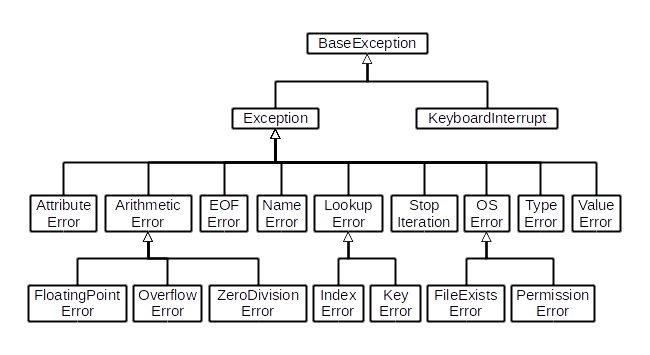
\includegraphics[scale=1.5]{images/python_exception_hierarchy.png}
    \end{adjustbox}
    \caption{Иерархия исключений в Python.}\label{fig:python-exception-hierarchy}
\end{figure}

За любым неудачным выделением памяти должен следовать вызов \texttt{PyErr\_NoMemory},
бросающий в интерпретатор исключение о нехватке памяти.
Для игнорирования исключений вызванных функций, внутренний контейнер интерпретатора должен
быть явно очищен от исключения вызовом функции \texttt{PyErr\_Clear}.
Использоваться она должна только если вызывающая функция не хочет уведомлять интерпретатор
о произошедшем исключении и готова обработать его самостоятельно.

В случае, если исключение происходит в критически-важных функциях, вроде <<опознания>>
PCI-устройства, требуется корректно уведомить об этом QEMU.

\subsection{Подход QEMU к обработке ошибок}\label{sec:ch2/sec2/sub5/sub1}

Модель ошибок в QEMU была, как и многое, вдохновлена моделью ошибок GLib.
В отличие от GLib, где класс исключения инкапсулирует в себе область, код ошибки и сообщение (\cref{fig:glib-error}),
класс исключения в QEMU более подробный (\cref{fig:qemu-error}) и помимо перечисленных полей содержит еще:
\begin{itemize}
    \item подсказку -- содержит дополнительную информацию, помимо сообщения;
    \item название файла и функции, в которых произошла ошибка;
    \item номер строки, где произошла ошибка.
\end{itemize}

\begin{figure}[!htbp]
    \centering
    \begin{adjustbox}{max totalsize={0.8\textwidth}{\textheight}}
        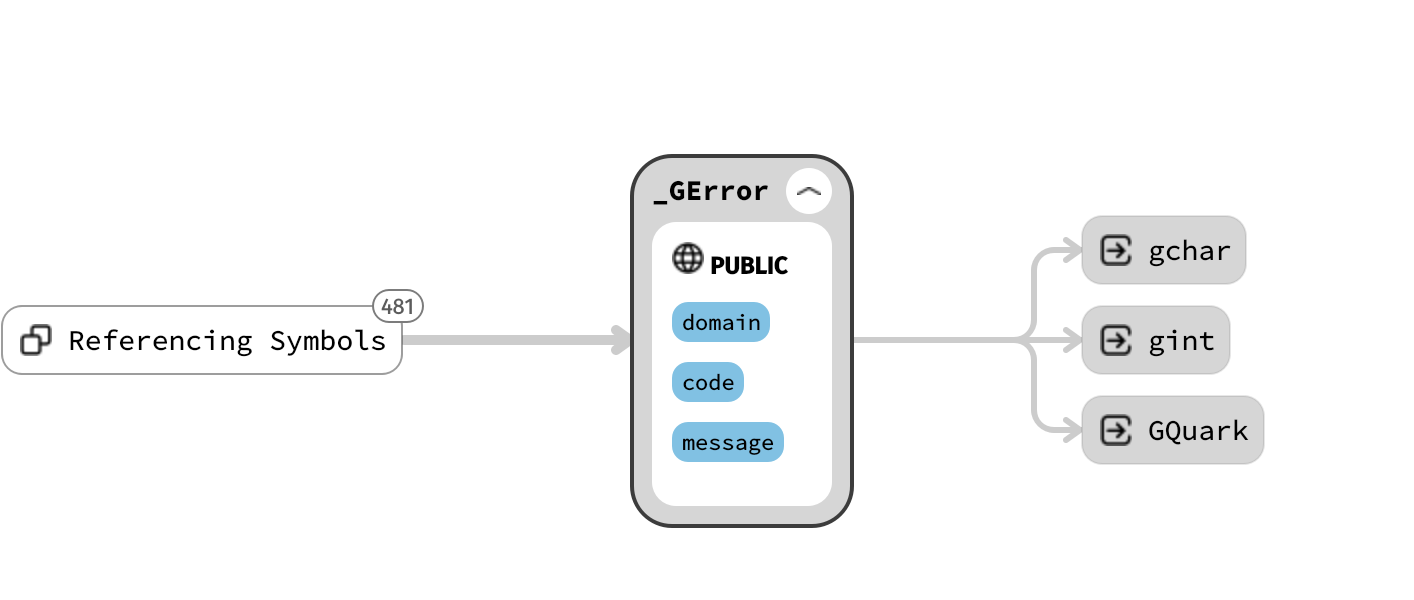
\includegraphics[]{images/glib-error.png}
    \end{adjustbox}
    \caption{Класс исключения в GLib.}\label{fig:glib-error}
\end{figure}

\begin{figure}[!htbp]
    \centering
    \begin{adjustbox}{max totalsize={0.8\textwidth}{\textheight}}
        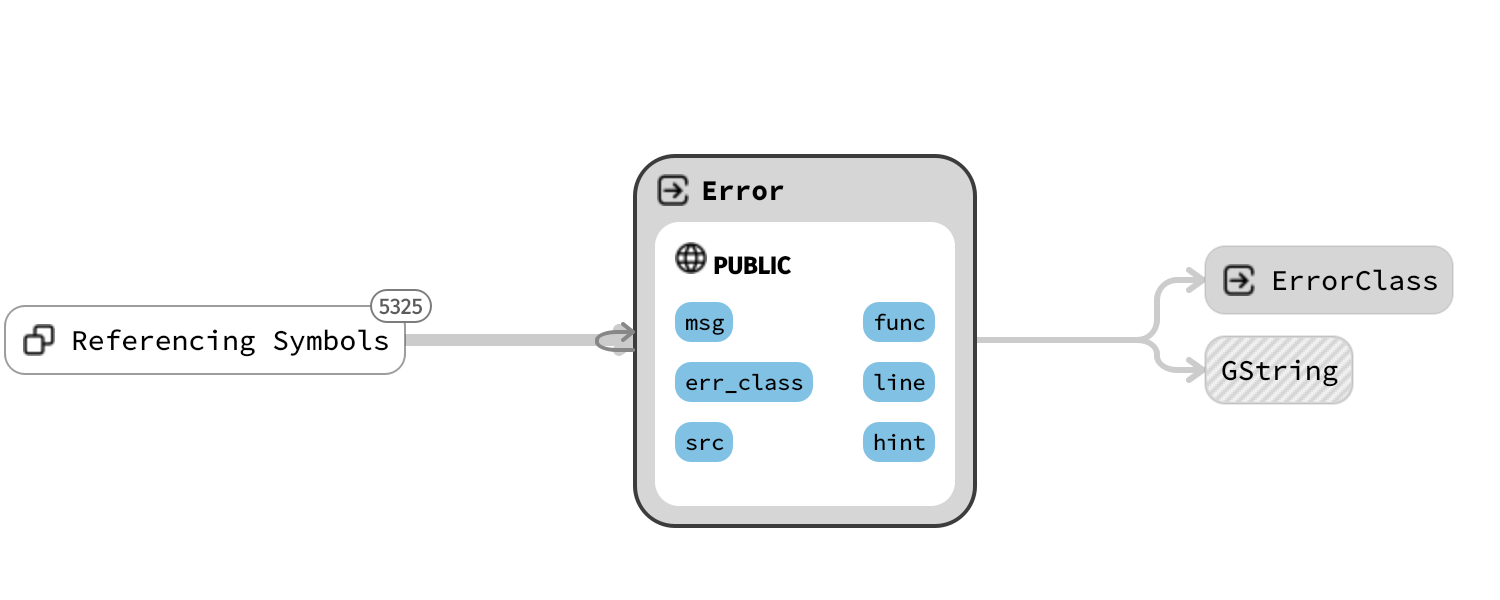
\includegraphics[]{images/qemu-error.png}
    \end{adjustbox}
    \caption{Класс исключения в QEMU.}\label{fig:qemu-error}
\end{figure}

Функция \texttt{error\_report} используется для уведомлении пользователя о
прозошедшей ошибке. В отличие от вызова функций печати стандартной библиотеки C,
данная функция, в случае подключенного монитора QEMU (средства управления QEMU
во время работы) выведет сообщение туда, а не в стандартный поток ошибок.

Для бросания ошибок используется макрос \texttt{error\_setg}, который инциализирует
исключение по переданному указателю. Передаваемое исключение должно быть одной из
двух глобальных переменных: \texttt{error\_abort}, \texttt{error\_fatal}.
В случае \texttt{error\_abort}, QEMU выводит сообщение исключения и вызывает
функцию \texttt{abort}, которая посылает работающему процессу (QEMU) сигнал
\texttt{SIGABRT}, вызывающий его экстренное завершение без дальнейшего вызова каких-либо
функций-деструкторов.
\texttt{error\_fatal} в свою очередь вызывает \texttt{exit}, что тоже вызывает
завершение работающего процесса, но с вызовом деструкторов, зарегистрированных
функцией \texttt{atexit}.

Все исключения внутри Python-логики должны быть обработаны. Если происходит
необработанное исключение внутри Python-кода, то функция \texttt{PyObject\_CallObject}
вернет \texttt{NULL} и выставит внутренний контейнер исключений.
В таком случае через \texttt{PyErr\_Fetch} будет получено сообщение произошедшего исключения,
на его основе будет вызвана функция \texttt{error\_setg} с ошибкой \texttt{error\_fatal},
которая корректно завершит работу QEMU.

\section{Компиляция Python-логики}\label{sec:ch2/sec2/sub6}

Python является интерпретируемым языком, но прежде чем выполниться,
код, компилируется в байт-код и уже потом исполняется на <<виртуальной машине>> Python.
Интерпретатор может оперировать в двух режимах: REPL и исполнение скриптов.
В первом случае, интерпретатор читает строка за строкой пользовательский
ввод, исполняя его как только сформируется корректная синтаксическая конструкция.
Во втором случае весь код, описанный в файле, первоначально компилируется в байткод и только потом исполняется
(\cref{fig:python-interpreter}).

\begin{figure}[!htbp]
    \centering
    \begin{adjustbox}{max totalsize={0.8\textwidth}{\textheight}}
        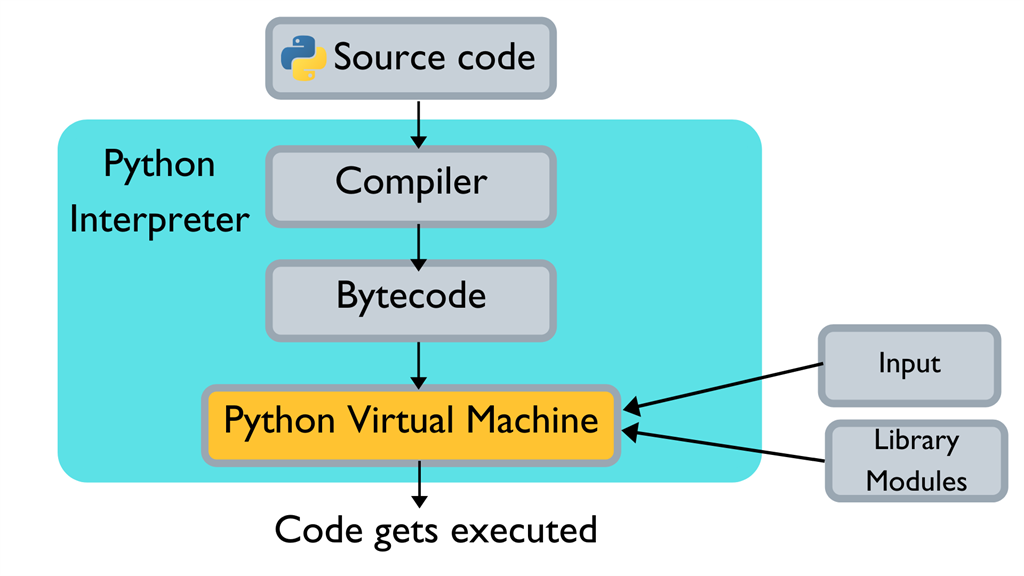
\includegraphics[]{images/python-interpreter.png}
    \end{adjustbox}
    \caption{Схема работы интерпретатора Python.}\label{fig:python-interpreter}
\end{figure}

Так как {\mylanguage} создает модуль QEMU, не зависящий от сторонних файлов
на диске (чтобы скомпилированная QEMU могла работать в любом окружении),
код с Python-логикой помещается в отдельный заголовочный файл, в котором
создается строковая переменная, его содержащая.
Данная строковая переменная компилируется во время класса устройства,
с помощью функции \texttt{Py\_CompileString}, создавая Python-модуль,
после чего Python-модуль импортируется в интерпретатор
через \texttt{PyImport\_ExecCodeModule}, позволяя запрашивать уже у модуля
функции логики устройства (\cref{fig:qemu-python-startup}).

\begin{figure}[!htbp]
    \centering
    \hspace*{-11.5cm}
    \begin{minipage}{10cm}
        
% !TEX encoding = UTF-8 Unicode
% Úτƒ-8 encoded
% http://www.linux.org.ru/forum/general/10357036
\tikzset{
    line/.style={draw, -latex'},
    every join/.style={line},
    u/.style={anchor=south},
    r/.style={anchor=west},
    fxd/.style={text width = 6em},
    it/.style={font={\small\itshape}},
    bf/.style={font={\small\bfseries}},
}
\tikzstyle{base_long} =
    [
        draw,
        on chain,
        on grid,
        align=center,
        minimum height=4ex,
        minimum width = 10ex,
        node distance = 6mm and 60mm,
        text badly centered,
    ]
\tikzstyle{base} =
    [
        draw,
        on chain,
        on grid,
        align=center,
        minimum height=4ex,
        minimum width = 10ex,
        node distance = 6mm and 60mm,
        text badly centered,
        text width=5cm
    ]
\tikzstyle{coord} =
    [
        coordinate,
        on chain,
        on grid
    ]
\tikzstyle{cloud} =
    [
        base,
        ellipse,
        node distance = 3cm,
        minimum height = 2em,
        text width=2cm
    ]
\tikzstyle{decision} =
    [
        base,
        diamond,
        aspect=2,
        node distance = 2cm,
        inner sep = 0pt
    ]
\tikzstyle{block} =
    [
        rectangle,
        base,
        %rounded corners,
        minimum height = 2em
    ]
\tikzstyle{print_block} =
    [
        base,
        tape,
        tape bend top=none,
    ]
\tikzstyle{io} =
    [
        base,
        trapezium,
        trapezium left angle = 70,
        trapezium right angle = 110,
    ]
\tikzstyle{prompt} =
    [
        base,
        trapezium,
        trapezium left angle = 90,
        trapezium right angle = 80,
        shape border rotate = 90
    ]
\tikzstyle{disk file} =
    [
        base,
        cylinder,
        aspect=0.2,
    ]
\tikzstyle{process} =
    [
        rectangle,
        base,
    ]
\makeatletter
\pgfkeys{/pgf/.cd,
    subrtshape w/.initial=2mm,
    cycleshape w/.initial=2mm
}
\pgfdeclareshape{parallelshape}{
    \inheritsavedanchors[from=rectangle]
    \inheritanchorborder[from=rectangle]
    \inheritanchor[from=rectangle]{north}
    \inheritanchor[from=rectangle]{center}
    \inheritanchor[from=rectangle]{west}
    \inheritanchor[from=rectangle]{east}
    \inheritanchor[from=rectangle]{mid}
    \inheritanchor[from=rectangle]{base}
    \inheritanchor[from=rectangle]{south}
    \backgroundpath{
        \southwest \pgf@xa=\pgf@x \pgf@ya=\pgf@y
        \northeast \pgf@xb=\pgf@x \pgf@yb=\pgf@y
        \def\ppd@offset{\pgfpoint{\pgfutil@tempdima}{0ex}}
        \def\ppd@offsetm{\pgfpoint{-\pgfutil@tempdima}{0ex}}
        \pgfpathmoveto{\pgfqpoint{\pgf@xa}{\pgf@ya}}
            \pgfpathlineto{\pgfqpoint{\pgf@xb}{\pgf@ya}}
        \pgfpathclose
        \pgfpathmoveto{\pgfqpoint{\pgf@xb}{\pgf@yb}}
            \pgfpathlineto{\pgfqpoint{\pgf@xa}{\pgf@yb}}
        \pgfpathclose
    }
}
\pgfdeclareshape{subrtshape}{
    \inheritsavedanchors[from=rectangle]
    \inheritanchorborder[from=rectangle]
    \inheritanchor[from=rectangle]{north}
    \inheritanchor[from=rectangle]{center}
    \inheritanchor[from=rectangle]{west}
    \inheritanchor[from=rectangle]{east}
    \inheritanchor[from=rectangle]{mid}
    \inheritanchor[from=rectangle]{base}
    \inheritanchor[from=rectangle]{south}
    \backgroundpath{
        \southwest \pgf@xa=\pgf@x \pgf@ya=\pgf@y
        \northeast \pgf@xb=\pgf@x \pgf@yb=\pgf@y
        \pgfmathsetlength\pgfutil@tempdima{\pgfkeysvalueof{/pgf/subrtshape w}}
        \def\ppd@offset{\pgfpoint{\pgfutil@tempdima}{0ex}}
        \def\ppd@offsetm{\pgfpoint{-\pgfutil@tempdima}{0ex}}
        \pgfpathmoveto{\pgfqpoint{\pgf@xa}{\pgf@ya}}
        \pgfpathlineto{\pgfqpoint{\pgf@xb}{\pgf@ya}}
        \pgfpathlineto{\pgfqpoint{\pgf@xb}{\pgf@yb}}
        \pgfpathlineto{\pgfqpoint{\pgf@xa}{\pgf@yb}}
        \pgfpathclose
        \pgfpathmoveto{\pgfpointadd{\pgfpoint{\pgf@xa}{\pgf@yb}}{\ppd@offsetm}}
        \pgfpathlineto{\pgfpointadd{\pgfpoint{\pgf@xa}{\pgf@ya}}{\ppd@offsetm}}
        \pgfpathlineto{\pgfpointadd{\pgfpoint{\pgf@xb}{\pgf@ya}}{\ppd@offset}}
        \pgfpathlineto{\pgfpointadd{\pgfpoint{\pgf@xb}{\pgf@yb}}{\ppd@offset}}
        \pgfpathclose
    }
}
\pgfdeclareshape{cyclebegshape}{
    \inheritsavedanchors[from=rectangle]
    \inheritanchorborder[from=rectangle]
    \inheritanchor[from=rectangle]{north}
    \inheritanchor[from=rectangle]{center}
    \inheritanchor[from=rectangle]{west}
    \inheritanchor[from=rectangle]{east}
    \inheritanchor[from=rectangle]{mid}
    \inheritanchor[from=rectangle]{base}
    \inheritanchor[from=rectangle]{south}
    \backgroundpath{
        \southwest \pgf@xa=\pgf@x \pgf@ya=\pgf@y
        \northeast \pgf@xb=\pgf@x \pgf@yb=\pgf@y
        \pgfmathsetlength\pgfutil@tempdima{\pgfkeysvalueof{/pgf/cycleshape w}}
        \pgfpathmoveto{\pgfqpoint{\pgf@xa}{\pgf@ya}}
\pgfpathlineto{\pgfpointadd{\pgfpoint{\pgf@xa}{\pgf@yb}}{\pgfpoint{0ex}{-\pgfutil@tempdima}}}
\pgfpathlineto{\pgfpointadd{\pgfpoint{\pgf@xa}{\pgf@yb}}{\pgfpoint{\pgfutil@tempdima}{0ex}}}
\pgfpathlineto{\pgfpointadd{\pgfpoint{\pgf@xb}{\pgf@yb}}{\pgfpoint{-\pgfutil@tempdima}{0ex}}}
\pgfpathlineto{\pgfpointadd{\pgfpoint{\pgf@xb}{\pgf@yb}}{\pgfpoint{0ex}{-\pgfutil@tempdima}}}
\pgfpathlineto{\pgfqpoint{\pgf@xb}{\pgf@ya}}
        \pgfpathclose
    }
}
\pgfdeclareshape{cycleendshape}{
    \inheritsavedanchors[from=rectangle]
    \inheritanchorborder[from=rectangle]
    \inheritanchor[from=rectangle]{north}
    \inheritanchor[from=rectangle]{center}
    \inheritanchor[from=rectangle]{west}
    \inheritanchor[from=rectangle]{east}
    \inheritanchor[from=rectangle]{mid}
    \inheritanchor[from=rectangle]{base}
    \inheritanchor[from=rectangle]{south}
    \backgroundpath{
        \southwest \pgf@xa=\pgf@x \pgf@ya=\pgf@y
        \northeast \pgf@xb=\pgf@x \pgf@yb=\pgf@y
        \pgfmathsetlength\pgfutil@tempdima{\pgfkeysvalueof{/pgf/cycleshape w}}
        \pgfpathmoveto{\pgfqpoint{\pgf@xb}{\pgf@yb}}
\pgfpathlineto{\pgfpointadd{\pgfpoint{\pgf@xb}{\pgf@ya}}{\pgfpoint{0ex}{\pgfutil@tempdima}}}
\pgfpathlineto{\pgfpointadd{\pgfpoint{\pgf@xb}{\pgf@ya}}{\pgfpoint{-\pgfutil@tempdima}{0ex}}}
\pgfpathlineto{\pgfpointadd{\pgfpoint{\pgf@xa}{\pgf@ya}}{\pgfpoint{\pgfutil@tempdima}{0ex}}}
\pgfpathlineto{\pgfpointadd{\pgfpoint{\pgf@xa}{\pgf@ya}}{\pgfpoint{0ex}{\pgfutil@tempdima}}}
\pgfpathlineto{\pgfqpoint{\pgf@xa}{\pgf@yb}}
        \pgfpathclose
    }
}
\makeatother
\tikzstyle{subroutine} =
    [
        base,
        subrtshape,
    ]
\tikzstyle{cyclebegin} =
    [
        base,
        cyclebegshape,
    ]
\tikzstyle{cycleend} =
    [
        base,
        cycleendshape,
    ]
\tikzstyle{connector} =
    [
        base,
        circle,
    ]

\tikzstyle{parallel} =
    [
        base_long,
        parallelshape,
    ]
\begin{tikzpicture}[%
    start chain=going below,    % General flow is top-to-bottom
    node distance=6mm and 30mm, % Global setup of box spacing
    ]

    \node [block]     (compilation)                              {\small Компиляция логики в байткод};
    \node [block]     (module)      [below = 2cm of compilation] {\small Создание Python-модуля из байткода};
    \node [io] (module var)  [below = 3cm of module]      {\small Переменная, хранящая Python-модуль с реализацией устройства};
    \node [process]   (func1)       [below = 3cm of module var]  {\small Функция, вызывающая логику};
    \node [process]   (func2)       [left = 6cm of func1]        {\small Функция, вызывающая логику};
    \node [process]   (func3)       [right = 6cm of func1]       {\small Функция, вызывающая логику};
    \node [rectangle] (etc left)    [left = 0.5cm of func2]        {\huge ...};
    \node [rectangle] (etc right)   [right = 0.5cm of func3]       {\huge ...};

    \draw [->] (compilation) -- (module);
    \draw [->] (module) -- (module var);
    \draw [->] (func1) -- (module var);
    \draw [->] (func2) -- (module var);
    \draw [->] (func3) -- (module var);

\end{tikzpicture}

    \end{minipage}
    \caption{Схема компиляции Python-логики устройства}\label{fig:qemu-python-startup}
\end{figure}


\section{Интеграция устройства в сборку QEMU}\label{sec:ch2/sec2/sub7}

После того, как файлы с исходным кодом устройства были сгенерированы, требуется
интегрировать устройство в сборку эмулятора QEMU (\cref{fig:qemu-compilation}).

Несмотря на то, что QEMU собирается meson'ом, в репозитории сохраняется
классический sh-скрипт конфигурации, вызвав который можно включить
или отключить компиляцию определенных устройств и возможностей QEMU.
Для добавления созданного устройства применяется шаблонизированный patch-файл,
в котором шаблонные значения препроцессируются и заменяются конкретными,
после чего patch накладывается на скрипт конфигурации.
Так как скрипт конфигурации постоянно и непредсказуемо может меняться,
то якорями для patch-файла являются неменяющийся код обработки ошибок
и добавление ключевых для компиляции QEMU библиотек (вроде GLib).

Скрипт конфигурации, который называется \texttt{configure} создается
файл \texttt{config-host.mak}, содержащий строки ключ-значение,
который загружается meson'ом и определяют, что именно добавлять в
результирующий исполняемый файл.

Так как логика устройства описана на языке Python, то интерпретатор Python
интегрируется в QEMU для ее исполнения, а компиляция устройства должна
проходить с соответствующими флагами. Для этого используется
скрипт, устанавливающийся вместе с Python -- \texttt{python3-config}.
Он позволяет запросить флаги для этапов компиляции (\texttt{--cflags})
и линковки (\texttt{--ldflags}) интерпретатора в программу.
Также используется флаг \texttt{--embed}, который указывает,
что Python на этапе будет встраиваться в программу.

\begin{figure}[!htbp]
    \centering
    
% !TEX encoding = UTF-8 Unicode
% Úτƒ-8 encoded
% http://www.linux.org.ru/forum/general/10357036
\tikzset{
    line/.style={draw, -latex'},
    every join/.style={line},
    u/.style={anchor=south},
    r/.style={anchor=west},
    fxd/.style={text width = 6em},
    it/.style={font={\small\itshape}},
    bf/.style={font={\small\bfseries}},
}
\tikzstyle{base_long} =
    [
        draw,
        on chain,
        on grid,
        align=center,
        minimum height=4ex,
        minimum width = 10ex,
        node distance = 6mm and 60mm,
        text badly centered,
    ]
\tikzstyle{base} =
    [
        draw,
        on chain,
        on grid,
        align=center,
        minimum height=4ex,
        minimum width = 10ex,
        node distance = 6mm and 60mm,
        text badly centered,
        text width=5cm
    ]
\tikzstyle{coord} =
    [
        coordinate,
        on chain,
        on grid
    ]
\tikzstyle{cloud} =
    [
        base,
        ellipse,
        node distance = 3cm,
        minimum height = 2em,
        text width=2cm
    ]
\tikzstyle{decision} =
    [
        base,
        diamond,
        aspect=2,
        node distance = 2cm,
        inner sep = 0pt
    ]
\tikzstyle{block} =
    [
        rectangle,
        base,
        rounded corners,
        minimum height = 2em
    ]
\tikzstyle{print_block} =
    [
        base,
        tape,
        tape bend top=none,
    ]
\tikzstyle{io} =
    [
        base,
        trapezium,
        trapezium left angle = 70,
        trapezium right angle = 110,
    ]
\tikzstyle{prompt} =
    [
        base,
        trapezium,
        trapezium left angle = 90,
        trapezium right angle = 80,
        shape border rotate = 90
    ]
\tikzstyle{disk file} =
    [
        base,
        cylinder,
        aspect=0.2,
    ]
\tikzstyle{process} =
    [
        rectangle,
        base,
    ]
\makeatletter
\pgfkeys{/pgf/.cd,
    subrtshape w/.initial=2mm,
    cycleshape w/.initial=2mm
}
\pgfdeclareshape{parallelshape}{
    \inheritsavedanchors[from=rectangle]
    \inheritanchorborder[from=rectangle]
    \inheritanchor[from=rectangle]{north}
    \inheritanchor[from=rectangle]{center}
    \inheritanchor[from=rectangle]{west}
    \inheritanchor[from=rectangle]{east}
    \inheritanchor[from=rectangle]{mid}
    \inheritanchor[from=rectangle]{base}
    \inheritanchor[from=rectangle]{south}
    \backgroundpath{
        \southwest \pgf@xa=\pgf@x \pgf@ya=\pgf@y
        \northeast \pgf@xb=\pgf@x \pgf@yb=\pgf@y
        \def\ppd@offset{\pgfpoint{\pgfutil@tempdima}{0ex}}
        \def\ppd@offsetm{\pgfpoint{-\pgfutil@tempdima}{0ex}}
        \pgfpathmoveto{\pgfqpoint{\pgf@xa}{\pgf@ya}}
            \pgfpathlineto{\pgfqpoint{\pgf@xb}{\pgf@ya}}
        \pgfpathclose
        \pgfpathmoveto{\pgfqpoint{\pgf@xb}{\pgf@yb}}
            \pgfpathlineto{\pgfqpoint{\pgf@xa}{\pgf@yb}}
        \pgfpathclose
    }
}
\pgfdeclareshape{subrtshape}{
    \inheritsavedanchors[from=rectangle]
    \inheritanchorborder[from=rectangle]
    \inheritanchor[from=rectangle]{north}
    \inheritanchor[from=rectangle]{center}
    \inheritanchor[from=rectangle]{west}
    \inheritanchor[from=rectangle]{east}
    \inheritanchor[from=rectangle]{mid}
    \inheritanchor[from=rectangle]{base}
    \inheritanchor[from=rectangle]{south}
    \backgroundpath{
        \southwest \pgf@xa=\pgf@x \pgf@ya=\pgf@y
        \northeast \pgf@xb=\pgf@x \pgf@yb=\pgf@y
        \pgfmathsetlength\pgfutil@tempdima{\pgfkeysvalueof{/pgf/subrtshape w}}
        \def\ppd@offset{\pgfpoint{\pgfutil@tempdima}{0ex}}
        \def\ppd@offsetm{\pgfpoint{-\pgfutil@tempdima}{0ex}}
        \pgfpathmoveto{\pgfqpoint{\pgf@xa}{\pgf@ya}}
        \pgfpathlineto{\pgfqpoint{\pgf@xb}{\pgf@ya}}
        \pgfpathlineto{\pgfqpoint{\pgf@xb}{\pgf@yb}}
        \pgfpathlineto{\pgfqpoint{\pgf@xa}{\pgf@yb}}
        \pgfpathclose
        \pgfpathmoveto{\pgfpointadd{\pgfpoint{\pgf@xa}{\pgf@yb}}{\ppd@offsetm}}
        \pgfpathlineto{\pgfpointadd{\pgfpoint{\pgf@xa}{\pgf@ya}}{\ppd@offsetm}}
        \pgfpathlineto{\pgfpointadd{\pgfpoint{\pgf@xb}{\pgf@ya}}{\ppd@offset}}
        \pgfpathlineto{\pgfpointadd{\pgfpoint{\pgf@xb}{\pgf@yb}}{\ppd@offset}}
        \pgfpathclose
    }
}
\pgfdeclareshape{cyclebegshape}{
    \inheritsavedanchors[from=rectangle]
    \inheritanchorborder[from=rectangle]
    \inheritanchor[from=rectangle]{north}
    \inheritanchor[from=rectangle]{center}
    \inheritanchor[from=rectangle]{west}
    \inheritanchor[from=rectangle]{east}
    \inheritanchor[from=rectangle]{mid}
    \inheritanchor[from=rectangle]{base}
    \inheritanchor[from=rectangle]{south}
    \backgroundpath{
        \southwest \pgf@xa=\pgf@x \pgf@ya=\pgf@y
        \northeast \pgf@xb=\pgf@x \pgf@yb=\pgf@y
        \pgfmathsetlength\pgfutil@tempdima{\pgfkeysvalueof{/pgf/cycleshape w}}
        \pgfpathmoveto{\pgfqpoint{\pgf@xa}{\pgf@ya}}
\pgfpathlineto{\pgfpointadd{\pgfpoint{\pgf@xa}{\pgf@yb}}{\pgfpoint{0ex}{-\pgfutil@tempdima}}}
\pgfpathlineto{\pgfpointadd{\pgfpoint{\pgf@xa}{\pgf@yb}}{\pgfpoint{\pgfutil@tempdima}{0ex}}}
\pgfpathlineto{\pgfpointadd{\pgfpoint{\pgf@xb}{\pgf@yb}}{\pgfpoint{-\pgfutil@tempdima}{0ex}}}
\pgfpathlineto{\pgfpointadd{\pgfpoint{\pgf@xb}{\pgf@yb}}{\pgfpoint{0ex}{-\pgfutil@tempdima}}}
\pgfpathlineto{\pgfqpoint{\pgf@xb}{\pgf@ya}}
        \pgfpathclose
    }
}
\pgfdeclareshape{cycleendshape}{
    \inheritsavedanchors[from=rectangle]
    \inheritanchorborder[from=rectangle]
    \inheritanchor[from=rectangle]{north}
    \inheritanchor[from=rectangle]{center}
    \inheritanchor[from=rectangle]{west}
    \inheritanchor[from=rectangle]{east}
    \inheritanchor[from=rectangle]{mid}
    \inheritanchor[from=rectangle]{base}
    \inheritanchor[from=rectangle]{south}
    \backgroundpath{
        \southwest \pgf@xa=\pgf@x \pgf@ya=\pgf@y
        \northeast \pgf@xb=\pgf@x \pgf@yb=\pgf@y
        \pgfmathsetlength\pgfutil@tempdima{\pgfkeysvalueof{/pgf/cycleshape w}}
        \pgfpathmoveto{\pgfqpoint{\pgf@xb}{\pgf@yb}}
\pgfpathlineto{\pgfpointadd{\pgfpoint{\pgf@xb}{\pgf@ya}}{\pgfpoint{0ex}{\pgfutil@tempdima}}}
\pgfpathlineto{\pgfpointadd{\pgfpoint{\pgf@xb}{\pgf@ya}}{\pgfpoint{-\pgfutil@tempdima}{0ex}}}
\pgfpathlineto{\pgfpointadd{\pgfpoint{\pgf@xa}{\pgf@ya}}{\pgfpoint{\pgfutil@tempdima}{0ex}}}
\pgfpathlineto{\pgfpointadd{\pgfpoint{\pgf@xa}{\pgf@ya}}{\pgfpoint{0ex}{\pgfutil@tempdima}}}
\pgfpathlineto{\pgfqpoint{\pgf@xa}{\pgf@yb}}
        \pgfpathclose
    }
}
\makeatother
\tikzstyle{subroutine} =
    [
        base,
        subrtshape,
    ]
\tikzstyle{cyclebegin} =
    [
        base,
        cyclebegshape,
    ]
\tikzstyle{cycleend} =
    [
        base,
        cycleendshape,
    ]
\tikzstyle{connector} =
    [
        base,
        circle,
    ]

\tikzstyle{parallel} =
    [
        base_long,
        parallelshape,
    ]
\begin{tikzpicture}[%
    start chain=going below,    % General flow is top-to-bottom
    node distance=6mm and 30mm, % Global setup of box spacing
    ]

    \node [cloud] (begin) {\small Начало};

    \node [process] (template convertation)
                    [below = 2cm of begin]
                    {\small Конвертация шаблона};

    \node [disk file] (template meson patch)
                      [left = 7cm of begin]
                      {\small Шаблон patch-файла для \texttt{meson}};
    \node [disk file] (template configure patch)
                      [below = 3cm of template meson patch]
                      {\small Шаблон patch-файла для \texttt{configure}};

    \coordinate (template between) at ($(template configure patch)!0.5!(template meson patch)$);


    \node [disk file] (configure patch)
                      [below = 3cm of template configure patch]
                      {\small Patch-файл для \texttt{configure}};
    \node [disk file] (meson patch)
                      [right = 6cm of template convertation]
                      {\small Patch-файл для \texttt{meson}};

    \node [process]   (patch application) [below = 3cm of template convertation] {\small Применение patch-файла};
    \node [subroutine] (cflags) [below = 3cm of patch application]         {\small Получение флагов компиляции интерпретатора};

    \node [process]   (build) [below = 3cm of cflags]   {\small Сборка};
    \node [disk file] (exe)   [right = 6cm of build]    {\small Исполняемый файл эмулятора};

    \node [cloud] (end) [below = 2cm of build]{\small Конец};

    \draw [->] (begin) -- (template convertation);
    \draw [->] (template configure patch) -- (template convertation.south west);
    \draw [->] (template meson patch) -- (template convertation.north west);
    \draw [->] (template convertation) -- (configure patch);
    \draw [->] (template convertation) -- (meson patch);
    \draw [->] (template convertation) -- (patch application);
    \draw [->] (configure patch) -- (patch application);
    \draw [->] (meson patch)     -- (patch application);
    \draw [->] (cflags) -- (build);
    \draw [->] (patch application) -- (cflags);
    \draw [->] (build) -- (exe);
    \draw [->] (build) -- (end);

\end{tikzpicture}

    \caption{Схема интеграции созданного устройства в QEMU.}\label{fig:qemu-compilation}
\end{figure}
